\documentclass[a4paper,12pt]{article}
\usepackage[utf8]{inputenc}
\usepackage[T1]{fontenc}
\usepackage[polish]{babel}
\usepackage{geometry}
\geometry{margin=1in}
\usepackage{amsmath, amssymb}
\usepackage{graphicx}
\usepackage{hyperref}
\usepackage{tabularx}

\begin{document}
\section{Zarządzanie pamięcią w języku C/C++}

\subsection{Wprowadzenie}
Zarządzanie pamięcią w językach C i C++ jest kluczowym aspektem programowania, ponieważ oba języki pozwalają na bezpośrednią kontrolę nad alokacją i dealokacją pamięci. Niewłaściwe zarządzanie pamięcią może prowadzić do wycieków pamięci, błędów segmentacji i nieprzewidywalnych zachowań programu.

\subsection{Rodzaje pamięci w C/C++}
W językach C i C++ można wyróżnić kilka obszarów pamięci:

\begin{itemize}
    \item \textbf{Pamięć statyczna} – zmienne globalne oraz zmienne zadeklarowane jako \texttt{static} są przechowywane w tej pamięci i istnieją przez cały czas działania programu.
    \item \textbf{Stos (stack)} – przechowuje zmienne lokalne oraz adresy powrotne funkcji. Pamięć na stosie jest automatycznie zwalniana po zakończeniu funkcji.
    \item \textbf{Sterta (heap)} – obszar pamięci przeznaczony do dynamicznej alokacji. Zarządzanie pamięcią na stercie jest odpowiedzialnością programisty.
\end{itemize}

\subsection{Alokacja i dealokacja pamięci w języku C}
W języku C dynamiczne zarządzanie pamięcią odbywa się za pomocą funkcji bibliotecznych z nagłówka \texttt{stdlib.h}:

\begin{itemize}
    \item \textbf{\texttt{malloc(size\_t size)}} – alokuje określoną ilość bajtów i zwraca wskaźnik do pierwszego bajtu tej pamięci. Nie inicjalizuje pamięci.
    \item \textbf{\texttt{calloc(size\_t num, size\_t size)}} – alokuje pamięć dla tablicy elementów i zeruje przydzieloną pamięć.
    \item \textbf{\texttt{realloc(void* ptr, size\_t new\_size)}} – zmienia rozmiar wcześniej zaalokowanego bloku pamięci.
    \item \textbf{\texttt{free(void* ptr)}} – zwalnia zaalokowaną pamięć.
\end{itemize}

\textbf{Przykład użycia funkcji \texttt{malloc} i \texttt{free}:}

\begin{verbatim}
#include <stdio.h>
#include <stdlib.h>

int main() {
    int *ptr = (int*) malloc(10 * sizeof(int)); // Alokacja tablicy 10 elementów
    if (ptr == NULL) {
        printf("Błąd alokacji pamięci\n");
        return 1;
    }
    free(ptr); // Zwolnienie pamięci
    return 0;
}
\end{verbatim}

\subsection{Alokacja i dealokacja pamięci w języku C++}
W języku C++ dynamiczne zarządzanie pamięcią odbywa się za pomocą operatorów:

\begin{itemize}
    \item \textbf{\texttt{new}} – alokuje pamięć dla pojedynczego obiektu lub tablicy.
    \item \textbf{\texttt{delete}} – zwalnia pamięć przydzieloną pojedynczemu obiektowi.
    \item \textbf{\texttt{delete[]}} – zwalnia pamięć przydzieloną tablicy.
\end{itemize}

\textbf{Przykład użycia \texttt{new} i \texttt{delete}:}

\begin{verbatim}
#include <iostream>

int main() {
    int *ptr = new int(10); // Alokacja pamięci dla pojedynczej liczby
    delete ptr; // Zwolnienie pamięci

    int *arr = new int[10]; // Alokacja pamięci dla tablicy
    delete[] arr; // Zwolnienie pamięci tablicy
    return 0;
}
\end{verbatim}

\subsection{Problemy związane z zarządzaniem pamięcią}
\begin{itemize}
    \item \textbf{Wycieki pamięci} – występują, gdy zaalokowana pamięć nie zostaje zwolniona.
    \item \textbf{Dereferencja pustego wskaźnika} – próba użycia wskaźnika o wartości \texttt{NULL} powoduje błąd wykonania.
    \item \textbf{Uszkodzenie pamięci} – zapisanie wartości poza przydzielonym obszarem może prowadzić do nieprzewidywalnych błędów.
    \item \textbf{Podwójne zwalnianie pamięci} – zwolnienie tej samej pamięci więcej niż raz może prowadzić do błędów.
\end{itemize}

\subsection{Mechanizmy zarządzania pamięcią w nowoczesnym C++}
Nowoczesny C++ (C++11 i nowsze) wprowadza inteligentne wskaźniki, które ułatwiają zarządzanie pamięcią:

\begin{itemize}
    \item \textbf{\texttt{std::unique\_ptr}} – zarządza pojedynczym obiektem i automatycznie zwalnia pamięć po zakończeniu jego żywotności.
    \item \textbf{\texttt{std::shared\_ptr}} – zarządza współdzieloną pamięcią i automatycznie zwalnia ją, gdy nie ma już żadnych referencji.
    \item \textbf{\texttt{std::weak\_ptr}} – słaby wskaźnik używany w celu uniknięcia cykli odniesień.
\end{itemize}

\textbf{Przykład użycia \texttt{std::unique\_ptr}:}

\begin{verbatim}
#include <iostream>
#include <memory>

int main() {
    std::unique_ptr<int> ptr = std::make_unique<int>(10);
    std::cout << *ptr << std::endl; // Wyświetla 10
    return 0; // Pamięć zostaje automatycznie zwolniona
}
\end{verbatim}

\subsection{Podsumowanie}
Zarządzanie pamięcią w językach C i C++ jest kluczowym aspektem programowania. Wymaga ono ostrożności i dbałości o poprawne zwalnianie pamięci. Nowoczesne mechanizmy, takie jak inteligentne wskaźniki w C++, znacząco ułatwiają pracę z pamięcią, redukując ryzyko błędów.

\section{Charakterystyka środowiska sprzętowego NVIDIA CUDA i modelu wykonania SIMT}

\subsection{Wprowadzenie}
CUDA (Compute Unified Device Architecture) to opracowana przez firmę NVIDIA platforma umożliwiająca wykorzystanie procesorów graficznych (GPU) do obliczeń równoległych. Środowisko sprzętowe CUDA charakteryzuje się specyficzną architekturą opartą na modelu równoległego wykonywania instrukcji SIMT (\textit{Single Instruction Multiple Threads}).

\subsection{Architektura sprzętowa NVIDIA CUDA}

Architektura sprzętowa CUDA opiera się na hierarchicznej organizacji zasobów obliczeniowych:
\begin{itemize}
    \item \textbf{GPU (Graphics Processing Unit)} – jednostka obliczeniowa zawierająca wiele multiprocesorów strumieniowych.
    \item \textbf{Multiprocesory strumieniowe (SM – Streaming Multiprocessor)} – podstawowe jednostki obliczeniowe GPU, zawierające zestawy rdzeni.
    \item \textbf{Rdzenie CUDA (CUDA Cores)} – elementarne jednostki wykonawcze realizujące operacje arytmetyczne i logiczne.
    \item \textbf{Warp} – grupa 32 wątków wykonywanych równocześnie w jednym SM.
    \item \textbf{Blok wątków (Thread Block)} – zestaw wątków współdzielących pamięć lokalną.
    \item \textbf{Siatka bloków (Grid of Blocks)} – zbiór bloków realizujących obliczenia w danym kernelu CUDA.
\end{itemize}

\begin{figure}[h]
    \centering
    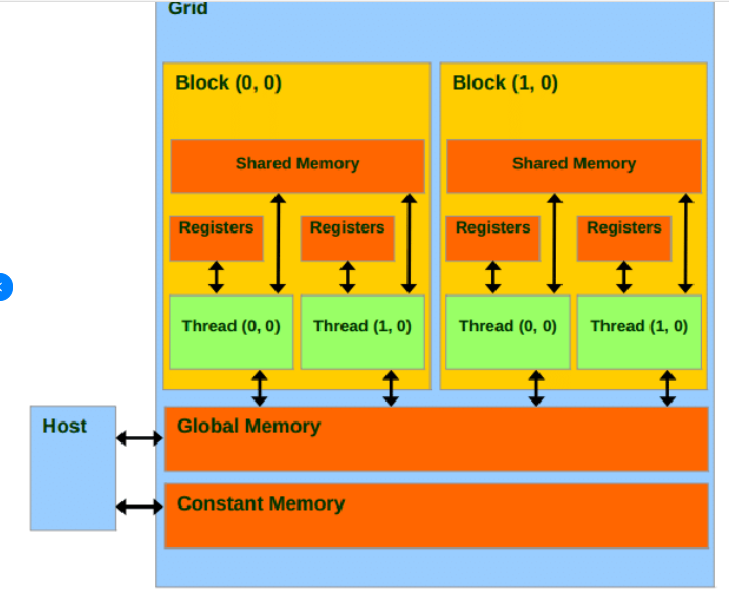
\includegraphics[width=0.7\textwidth]{cuda_architecture.png}
    \caption{Hierarchiczna organizacja zasobów CUDA.}
\end{figure}

\subsection{Model wykonania SIMT (Single Instruction Multiple Threads)}

Model \textbf{SIMT} stosowany w architekturze CUDA polega na jednoczesnym wykonywaniu tej samej instrukcji przez wiele wątków.

\textbf{Cechy SIMT:}
\begin{itemize}
    \item Każdy multiprocesor SM wykonuje wiele wątków równocześnie.
    \item Wątki w ramach jednego warpa (32 wątki) wykonują te same instrukcje, ale na różnych danych.
    \item Gdy występuje rozgałęzienie warunkowe, wątki w warpie mogą wykonywać różne ścieżki kodu (\textit{thread divergence}), co prowadzi do spadku wydajności.
\end{itemize}

\subsection{Struktura wykonania w CUDA}

\subsubsection{1. Hierarchia wątków w modelu CUDA}
\begin{itemize}
    \item \textbf{Wątek (Thread)} – jednostka wykonawcza pracująca na określonych danych.
    \item \textbf{Blok wątków (Thread Block)} – grupa wątków, które mogą współdzielić pamięć współdzieloną.
    \item \textbf{Siatka bloków (Grid of Blocks)} – zestaw bloków, które wykonują równoległe obliczenia.
\end{itemize}

\textbf{Przykład konfiguracji siatki i bloków:}
\begin{verbatim}
kernel<<<numBlocks, threadsPerBlock>>>(d_data);
\end{verbatim}

\subsubsection{2. Organizacja pamięci w CUDA}
CUDA udostępnia różne rodzaje pamięci:
\begin{itemize}
    \item \textbf{Pamięć rejestrów} – najszybsza, ale ograniczona ilościowo.
    \item \textbf{Pamięć współdzielona (Shared Memory)} – szybka pamięć dostępna w obrębie jednego bloku wątków.
    \item \textbf{Pamięć globalna (Global Memory)} – dostępna dla wszystkich wątków, ale o dużym opóźnieniu.
    \item \textbf{Pamięć stała (Constant Memory)} – zoptymalizowana dla niezmiennych danych.
    \item \textbf{Pamięć tekstur i powierzchni (Texture \& Surface Memory)} – wykorzystywana w operacjach graficznych i analizie obrazu.
\end{itemize}

\subsection{Przykładowa implementacja kernela CUDA}
Przykład prostego kernela sumującego dwa wektory:
\begin{verbatim}
__global__ void addVectors(int *a, int *b, int *c, int n) {
    int idx = threadIdx.x + blockIdx.x * blockDim.x;
    if (idx < n) {
        c[idx] = a[idx] + b[idx];
    }
}
\end{verbatim}

\subsection{Zalety i ograniczenia modelu SIMT}

\textbf{Zalety:}
\begin{itemize}
    \item Wysoka wydajność w obliczeniach masowo-równoległych.
    \item Efektywne wykorzystanie zasobów sprzętowych GPU.
    \item Redukcja czasu obliczeń w porównaniu do CPU.
\end{itemize}

\textbf{Ograniczenia:}
\begin{itemize}
    \item Problemy z \textit{thread divergence}, gdy wątki wykonują różne ścieżki kodu.
    \item Konieczność optymalizacji dostępu do pamięci globalnej.
    \item Wysokie wymagania pamięciowe przy dużych rozmiarach danych.
\end{itemize}

\subsection{Podsumowanie}
\begin{itemize}
    \item CUDA pozwala na programowanie GPU z wykorzystaniem hierarchii wątków.
    \item Model SIMT umożliwia jednoczesne wykonywanie tej samej instrukcji przez wiele wątków.
    \item Optymalizacja pamięci i unikanie \textit{thread divergence} są kluczowe dla efektywnego programowania CUDA.
    \item CUDA znajduje zastosowanie w obliczeniach naukowych, sztucznej inteligencji i grafice komputerowej.
\end{itemize}

\section{Rola i umiejscowienie wywołań systemowych w architekturze systemu operacyjnego, sposób ich uruchamiania, przykłady wywołania}

\subsection{Wprowadzenie}
Wywołania systemowe (ang. \textit{system calls}) to interfejs umożliwiający programom użytkownika komunikację z jądrem systemu operacyjnego. Zapewniają dostęp do zasobów sprzętowych i funkcji systemowych w kontrolowany sposób.

\subsection{Rola wywołań systemowych}
Wywołania systemowe pełnią kluczową rolę w operacjach takich jak:
\begin{itemize}
    \item Zarządzanie procesami (tworzenie, synchronizacja, zakończenie).
    \item Obsługa plików (otwieranie, zamykanie, czytanie, zapis).
    \item Komunikacja międzyprocesowa (IPC).
    \item Zarządzanie pamięcią (alokacja, zwalnianie).
    \item Obsługa urządzeń wejścia/wyjścia.
    \item Sieciowa komunikacja.
\end{itemize}

\subsection{Umiejscowienie wywołań systemowych w architekturze systemu operacyjnego}
W architekturze systemu operacyjnego wywołania systemowe działają na granicy przestrzeni użytkownika (\textit{user space}) i przestrzeni jądra (\textit{kernel space}).

\begin{itemize}
    \item \textbf{Przestrzeń użytkownika} – zawiera procesy aplikacji, które nie mają bezpośredniego dostępu do sprzętu.
    \item \textbf{Przestrzeń jądra} – kontroluje zasoby sprzętowe i wykonuje operacje niskopoziomowe.
    \item \textbf{Interfejs wywołań systemowych} – działa jako pośrednik, przekazując żądania użytkownika do jądra.
\end{itemize}

\subsection{Sposób uruchamiania wywołań systemowych}
Wywołania systemowe są wywoływane przez aplikacje użytkownika w następujący sposób:
\begin{enumerate}
    \item Aplikacja użytkownika wywołuje funkcję biblioteczną (np. \texttt{open()} w języku C).
    \item Funkcja biblioteczna przekazuje żądanie do jądra poprzez instrukcję pułapki (ang. \textit{trap}).
    \item Jądro przełącza kontekst na przestrzeń jądra i wykonuje odpowiednią funkcję.
    \item Wynik jest zwracany do aplikacji użytkownika.
\end{enumerate}

\textbf{Schemat przepływu wywołania systemowego:}
\begin{verbatim}
Program użytkownika → Biblioteka standardowa → Przerwanie → Jądro OS → Wynik
\end{verbatim}

\subsection{Przykłady wywołań systemowych}

\subsubsection{1. Wywołania systemowe do obsługi plików}
\begin{itemize}
    \item \textbf{open()} – otwiera plik.
    \item \textbf{read()} – odczytuje dane z pliku.
    \item \textbf{write()} – zapisuje dane do pliku.
    \item \textbf{close()} – zamyka plik.
\end{itemize}

\textbf{Przykład w języku C:}
\begin{verbatim}
int fd = open("plik.txt", O_RDONLY);
read(fd, buffer, sizeof(buffer));
close(fd);
\end{verbatim}

\subsubsection{2. Wywołania systemowe do zarządzania procesami}
\begin{itemize}
    \item \textbf{fork()} – tworzy nowy proces.
    \item \textbf{exec()} – uruchamia nowy program w bieżącym procesie.
    \item \textbf{wait()} – czeka na zakończenie procesu potomnego.
    \item \textbf{exit()} – kończy działanie procesu.
\end{itemize}

\textbf{Przykład użycia \texttt{fork()}:}
\begin{verbatim}
pid_t pid = fork();
if (pid == 0) {
    printf("Proces potomny\n");
} else {
    printf("Proces macierzysty\n");
}
\end{verbatim}

\subsubsection{3. Wywołania systemowe do zarządzania pamięcią}
\begin{itemize}
    \item \textbf{mmap()} – mapuje plik lub pamięć do przestrzeni adresowej.
    \item \textbf{brk()} – dynamicznie zmienia rozmiar sterty procesu.
\end{itemize}

\textbf{Przykład użycia \texttt{mmap()}:}
\begin{verbatim}
void *ptr = mmap(NULL, 4096, PROT_READ | PROT_WRITE, MAP_PRIVATE | MAP_ANONYMOUS, -1, 0);
\end{verbatim}

\subsubsection{4. Wywołania systemowe do komunikacji międzyprocesowej}
\begin{itemize}
    \item \textbf{pipe()} – tworzy kanał komunikacyjny między procesami.
    \item \textbf{shmget()} – tworzy segment pamięci współdzielonej.
    \item \textbf{socket()} – tworzy gniazdo komunikacyjne.
\end{itemize}

\subsection{Podsumowanie}
\begin{itemize}
    \item Wywołania systemowe są podstawowym mechanizmem komunikacji między aplikacjami a jądrem systemu operacyjnego.
    \item Są używane do zarządzania plikami, procesami, pamięcią oraz komunikacją międzyprocesową.
    \item Wywołania systemowe przechodzą z przestrzeni użytkownika do przestrzeni jądra, zapewniając kontrolowany dostęp do zasobów systemowych.
\end{itemize}

\section{Główne wzorce architektoniczne oprogramowania}

\subsection{Wprowadzenie}
Wzorce architektoniczne definiują wysokopoziomowe struktury organizacyjne systemów oprogramowania. Określają sposób podziału systemu na komponenty oraz ich interakcje, co pozwala na efektywne projektowanie skalowalnych, elastycznych i łatwych w utrzymaniu aplikacji.

\subsection{Podstawowe wzorce architektoniczne}

\subsubsection{1. Architektura warstwowa (Layered Architecture)}
\textbf{Opis:}  
System podzielony jest na warstwy, z których każda realizuje określoną funkcjonalność i komunikuje się z warstwami sąsiednimi.

\textbf{Struktura:}
\begin{itemize}
    \item Warstwa prezentacji – interfejs użytkownika.
    \item Warstwa logiki biznesowej – przetwarzanie danych i reguły aplikacji.
    \item Warstwa dostępu do danych – komunikacja z bazą danych.
    \item Warstwa danych – baza danych i systemy przechowywania informacji.
\end{itemize}

\textbf{Zalety:}
\begin{itemize}
    \item Modularność i łatwość testowania.
    \item Możliwość oddzielenia interfejsu od logiki biznesowej.
\end{itemize}

\textbf{Wady:}
\begin{itemize}
    \item Może prowadzić do spadku wydajności z powodu licznych warstw pośrednich.
\end{itemize}

\subsubsection{2. Architektura klient-serwer (Client-Server)}
\textbf{Opis:}  
System podzielony jest na dwa główne komponenty: klienta, który żąda usług, oraz serwer, który te usługi udostępnia.

\textbf{Zastosowanie:}
\begin{itemize}
    \item Aplikacje internetowe (np. HTTP, REST API).
    \item Systemy baz danych (np. MySQL, PostgreSQL).
\end{itemize}

\textbf{Zalety:}
\begin{itemize}
    \item Centralizacja logiki aplikacji na serwerze.
    \item Łatwa aktualizacja klienta bez wpływu na serwer.
\end{itemize}

\textbf{Wady:}
\begin{itemize}
    \item Wysokie obciążenie serwera przy dużej liczbie użytkowników.
\end{itemize}

\subsubsection{3. Architektura mikroserwisowa (Microservices)}
\textbf{Opis:}  
System składa się z wielu niezależnych usług (mikroserwisów), które komunikują się przez API.

\textbf{Zastosowanie:}
\begin{itemize}
    \item Aplikacje chmurowe i rozproszone.
    \item Duże systemy internetowe (np. Netflix, Amazon).
\end{itemize}

\textbf{Zalety:}
\begin{itemize}
    \item Skalowalność i łatwość wdrażania poszczególnych komponentów.
    \item Możliwość użycia różnych technologii w różnych mikroserwisach.
\end{itemize}

\textbf{Wady:}
\begin{itemize}
    \item Złożoność zarządzania komunikacją między usługami.
\end{itemize}

\subsubsection{4. Architektura zdarzeniowa (Event-Driven Architecture)}
\textbf{Opis:}  
Komponenty systemu komunikują się poprzez zdarzenia asynchroniczne.

\textbf{Zastosowanie:}
\begin{itemize}
    \item Systemy czasu rzeczywistego (np. IoT, giełda papierów wartościowych).
\end{itemize}

\textbf{Zalety:}
\begin{itemize}
    \item Wysoka responsywność i skalowalność.
\end{itemize}

\textbf{Wady:}
\begin{itemize}
    \item Złożoność obsługi komunikacji i zarządzania stanem.
\end{itemize}

\subsubsection{5. Architektura model-widok-kontroler (MVC – Model-View-Controller)}
\textbf{Opis:}  
System podzielony na trzy komponenty:
\begin{itemize}
    \item \textbf{Model} – logika biznesowa i dane.
    \item \textbf{Widok (View)} – interfejs użytkownika.
    \item \textbf{Kontroler (Controller)} – obsługuje interakcje użytkownika.
\end{itemize}

\textbf{Zastosowanie:}
\begin{itemize}
    \item Aplikacje internetowe (np. frameworki jak Django, Spring MVC).
\end{itemize}

\textbf{Zalety:}
\begin{itemize}
    \item Oddzielenie warstw poprawia organizację kodu.
\end{itemize}

\textbf{Wady:}
\begin{itemize}
    \item Może prowadzić do złożoności w większych systemach.
\end{itemize}

\subsubsection{6. Architektura repozytorium (Repository Architecture)}
\textbf{Opis:}  
System składa się z centralnego repozytorium danych, z którego korzystają wszystkie komponenty.

\textbf{Zastosowanie:}
\begin{itemize}
    \item Kompilatory (np. GCC).
    \item Systemy zarządzania wiedzą.
\end{itemize}

\textbf{Zalety:}
\begin{itemize}
    \item Spójność danych w całym systemie.
\end{itemize}

\textbf{Wady:}
\begin{itemize}
    \item Możliwy wąskie gardło w dostępie do repozytorium.
\end{itemize}

\subsubsection{7. Architektura rurek i filtrów (Pipe-and-Filter)}
\textbf{Opis:}  
System składa się z przetwarzających dane komponentów (\textit{filtrów}), które są połączone kanałami przepływu danych (\textit{rurkami}).

\textbf{Zastosowanie:}
\begin{itemize}
    \item Przetwarzanie strumieni danych (np. potok w systemach UNIX).
\end{itemize}

\textbf{Zalety:}
\begin{itemize}
    \item Możliwość łatwego komponowania procesów.
\end{itemize}

\textbf{Wady:}
\begin{itemize}
    \item Może powodować wysoką latencję przy dużych zbiorach danych.
\end{itemize}

\subsection{Podsumowanie}
\begin{itemize}
    \item Wzorce architektoniczne pomagają w organizacji systemów oprogramowania.
    \item Architektura warstwowa jest klasyczna i szeroko stosowana.
    \item Mikroserwisy i architektura zdarzeniowa są preferowane w nowoczesnych, skalowalnych systemach.
    \item Wybór wzorca zależy od wymagań projektu, wydajności i skalowalności systemu.
\end{itemize}

\section{Refaktoryzacja oprogramowania i wybrane jej sposoby}

\subsection{Wprowadzenie}
Refaktoryzacja oprogramowania to proces restrukturyzacji kodu w celu poprawy jego jakości, czytelności i utrzymania, bez zmiany zewnętrznego zachowania programu. Jest kluczowa dla długoterminowej efektywności projektu i zapobiega zjawisku długu technologicznego.

\subsection{Cele refaktoryzacji}
\begin{itemize}
    \item Poprawa czytelności i zrozumiałości kodu.
    \item Zmniejszenie złożoności i redundancji.
    \item Ułatwienie przyszłego rozwoju i utrzymania systemu.
    \item Poprawa wydajności poprzez eliminację zbędnych operacji.
    \item Zwiększenie testowalności i redukcja błędów.
\end{itemize}

\subsection{Podstawowe techniki refaktoryzacji}

\subsubsection{1. Ekstrakcja metod (\textit{Extract Method})}
Polega na wydzieleniu fragmentu kodu do nowej metody w celu zwiększenia czytelności i unikania duplikacji.

\textbf{Przykład przed refaktoryzacją:}
\begin{verbatim}
void oblicz() {
    int suma = 0;
    for (int i = 0; i < lista.size(); i++) {
        suma += lista[i];
    }
    System.out.println("Suma: " + suma);
}
\end{verbatim}

\textbf{Po refaktoryzacji:}
\begin{verbatim}
void oblicz() {
    int suma = sumujElementy();
    System.out.println("Suma: " + suma);
}

int sumujElementy() {
    int suma = 0;
    for (int i = 0; i < lista.size(); i++) {
        suma += lista[i];
    }
    return suma;
}
\end{verbatim}

\subsubsection{2. Zastąpienie magicznych liczb stałymi (\textit{Replace Magic Number with Constant})}
Pozwala uniknąć nieczytelnych wartości liczbowych w kodzie.

\textbf{Przed:}
\begin{verbatim}
double obliczObwod(double promien) {
    return 2 * 3.14159 * promien;
}
\end{verbatim}

\textbf{Po:}
\begin{verbatim}
static final double PI = 3.14159;

double obliczObwod(double promien) {
    return 2 * PI * promien;
}
\end{verbatim}

\subsubsection{3. Wprowadzenie obiektu parametru (\textit{Introduce Parameter Object})}
Zamiast przekazywać wiele argumentów, można przekazać obiekt enkapsulujący dane.

\textbf{Przed:}
\begin{verbatim}
void ustawWymiary(int szerokosc, int wysokosc, int glebokosc) { ... }
\end{verbatim}

\textbf{Po:}
\begin{verbatim}
class Wymiary {
    int szerokosc, wysokosc, glebokosc;
}

void ustawWymiary(Wymiary wymiary) { ... }
\end{verbatim}

\subsubsection{4. Usunięcie zbędnych komentarzy}
Czysty kod powinien być samodokumentujący się, a nadmiar komentarzy może świadczyć o złej jakości kodu.

\textbf{Przed:}
\begin{verbatim}
// Dodaje produkt do listy
listaProduktow.add(produkt);
\end{verbatim}

\textbf{Po:}
\begin{verbatim}
dodajProduktDoListy(produkt);
\end{verbatim}

\subsubsection{5. Podział dużych klas (\textit{Extract Class})}
Jeśli klasa ma zbyt wiele odpowiedzialności, warto podzielić ją na mniejsze.

\textbf{Przed:}
\begin{verbatim}
class Zamowienie {
    List<Produkt> produkty;
    double obliczCene() { ... }
    void wyslijEmailPotwierdzajacy() { ... }
}
\end{verbatim}

\textbf{Po podziale:}
\begin{verbatim}
class Zamowienie {
    List<Produkt> produkty;
    double obliczCene() { ... }
}

class Notyfikacja {
    void wyslijEmailPotwierdzajacy() { ... }
}
\end{verbatim}

\subsection{Automatyzacja refaktoryzacji}
Wiele narzędzi wspiera refaktoryzację, np.:
\begin{itemize}
    \item IntelliJ IDEA, Eclipse – refaktoryzacja kodu w językach obiektowych.
    \item SonarQube – analiza jakości kodu.
    \item Black, Prettier – formatowanie kodu w Pythonie i JavaScript.
\end{itemize}

\subsection{Podsumowanie}
\begin{itemize}
    \item Refaktoryzacja poprawia jakość kodu i ułatwia jego utrzymanie.
    \item Wprowadzenie metod, eliminacja magicznych liczb i podział dużych klas zwiększają czytelność.
    \item Nowoczesne narzędzia wspomagają proces refaktoryzacji.
    \item Regularna refaktoryzacja zmniejsza ryzyko długu technologicznego.
\end{itemize}

\section{Mechanizmy przesyłania komunikatów w systemach rozproszonych}

\subsection{Wprowadzenie}
Systemy rozproszone składają się z wielu węzłów komunikujących się poprzez sieć. Podstawowym mechanizmem wymiany informacji między procesami jest przesyłanie komunikatów (\textit{message passing}). Efektywna komunikacja w systemach rozproszonych wymaga mechanizmów zapewniających niezawodność, synchronizację i efektywne zarządzanie przesyłanymi danymi.

\subsection{Podstawowe modele komunikacji}

\subsubsection{1. Komunikacja synchroniczna i asynchroniczna}
\begin{itemize}
    \item \textbf{Komunikacja synchroniczna} – nadawca czeka na potwierdzenie odbioru komunikatu przed kontynuacją pracy.
    \item \textbf{Komunikacja asynchroniczna} – nadawca wysyła komunikat i natychmiast kontynuuje działanie, a odbiorca może go odebrać później.
\end{itemize}

\textbf{Zastosowanie:}
\begin{itemize}
    \item Synchroniczna – systemy wymagające spójności, np. systemy bankowe.
    \item Asynchroniczna – systemy wymagające wysokiej przepustowości, np. przesyłanie wiadomości w mediach społecznościowych.
\end{itemize}

\subsubsection{2. Komunikacja jednokierunkowa i dwukierunkowa}
\begin{itemize}
    \item \textbf{Jednokierunkowa (Unidirectional)} – komunikacja odbywa się w jednym kierunku (np. \textit{UDP}).
    \item \textbf{Dwukierunkowa (Bidirectional)} – komunikacja wymaga odpowiedzi od odbiorcy (np. \textit{TCP}).
\end{itemize}

\subsubsection{3. Komunikacja jedno-do-jednego i jedno-do-wielu}
\begin{itemize}
    \item \textbf{Jedno-do-jednego (point-to-point)} – komunikacja między dwoma procesami.
    \item \textbf{Jedno-do-wielu (multicast, broadcast)} – komunikacja do wielu procesów jednocześnie.
\end{itemize}

\subsection{Mechanizmy przesyłania komunikatów}

\subsubsection{1. Gniazda (Sockets)}
Gniazda to podstawowy mechanizm komunikacji między procesami w sieci.

\textbf{Rodzaje gniazd:}
\begin{itemize}
    \item \textbf{Gniazda strumieniowe (TCP)} – zapewniają niezawodny, uporządkowany przesył danych.
    \item \textbf{Gniazda datagramowe (UDP)} – zapewniają szybki, ale niegwarantowany przesył danych.
\end{itemize}

\textbf{Przykład kodu w C (gniazdo TCP):}
\begin{verbatim}
int sockfd = socket(AF_INET, SOCK_STREAM, 0);
connect(sockfd, (struct sockaddr*)&server_addr, sizeof(server_addr));
send(sockfd, message, strlen(message), 0);
\end{verbatim}

\subsubsection{2. Kolejki komunikatów (Message Queues)}
Mechanizm kolejek pozwala na przechowywanie i odbieranie komunikatów asynchronicznie.

\textbf{Popularne implementacje:}
\begin{itemize}
    \item \textbf{POSIX Message Queues} – standard w systemach UNIX.
    \item \textbf{RabbitMQ, Apache Kafka} – systemy kolejkowania komunikatów w systemach rozproszonych.
\end{itemize}

\subsubsection{3. Pamięć współdzielona}
Procesy mogą wymieniać dane poprzez wspólną przestrzeń adresową.

\textbf{Zalety:}
\begin{itemize}
    \item Bardzo szybka wymiana danych.
    \item Unikanie narzutu komunikacyjnego sieci.
\end{itemize}

\textbf{Wady:}
\begin{itemize}
    \item Wymaga synchronizacji dostępu (semafory, muteksy).
    \item Ograniczona do systemów działających na jednym węźle.
\end{itemize}

\subsubsection{4. Remote Procedure Call (RPC)}
RPC pozwala na wywoływanie funkcji na zdalnym komputerze tak, jakby były lokalne.

\textbf{Przykłady technologii:}
\begin{itemize}
    \item \textbf{gRPC} – nowoczesne RPC oparte na HTTP/2.
    \item \textbf{XML-RPC, JSON-RPC} – lekkie protokoły RPC.
\end{itemize}

\textbf{Przykład RPC w Pythonie (gRPC):}
\begin{verbatim}
import grpc
channel = grpc.insecure_channel('localhost:50051')
response = stub.MethodName(request)
\end{verbatim}

\subsubsection{5. Publish-Subscribe (Pub/Sub)}
Wzorzec komunikacyjny, w którym nadawca (\textit{publisher}) wysyła komunikaty do kanału, a subskrybenci (\textit{subscribers}) je odbierają.

\textbf{Przykłady implementacji:}
\begin{itemize}
    \item \textbf{Apache Kafka} – skalowalna platforma do przesyłania strumieni danych.
    \item \textbf{MQTT} – protokół komunikacji w IoT.
\end{itemize}

\subsubsection{6. Strumieniowanie komunikatów (Message Streaming)}
Mechanizm umożliwia przesyłanie dużych ilości danych w czasie rzeczywistym.

\textbf{Przykłady implementacji:}
\begin{itemize}
    \item \textbf{Apache Kafka, Apache Pulsar} – rozproszone przetwarzanie strumieniowe.
    \item \textbf{Google Cloud Pub/Sub} – system do strumieniowego przesyłania danych w chmurze.
\end{itemize}

\subsection{Porównanie mechanizmów przesyłania komunikatów}

\begin{table}[h]
    \centering
    \renewcommand{\arraystretch}{1.3} % Poprawia czytelność tabeli
    \begin{tabularx}{\textwidth}{|l|X|X|}
        \hline
        \textbf{Mechanizm} & \textbf{Zalety} & \textbf{Wady} \\
        \hline
        \textbf{Gniazda (Sockets)} & Niski narzut, szybka komunikacja & Wymaga zarządzania połączeniami \\
        \hline
        \textbf{Kolejki komunikatów} & Buforowanie komunikatów & Większe opóźnienia \\
        \hline
        \textbf{Pamięć współdzielona} & Najszybsza wymiana danych & Ograniczona do jednego systemu \\
        \hline
        \textbf{RPC} & Transparentność wywołań & Opóźnienia sieciowe \\
        \hline
        \textbf{Publish-Subscribe} & Łatwa skalowalność & Opóźnienia propagacji \\
        \hline
        \textbf{Strumieniowanie} & Przetwarzanie w czasie rzeczywistym & Złożoność implementacji \\
        \hline
    \end{tabularx}
    \caption{Porównanie mechanizmów przesyłania komunikatów}
\end{table}


\subsection{Podsumowanie}
\begin{itemize}
    \item Przesyłanie komunikatów w systemach rozproszonych może odbywać się synchronicznie lub asynchronicznie.
    \item Gniazda są podstawowym mechanizmem komunikacji w sieci.
    \item Kolejki komunikatów i strumieniowanie danych zapewniają niezależność nadawcy i odbiorcy.
    \item RPC upraszcza wywołania zdalnych funkcji, a Pub/Sub umożliwia komunikację wielu węzłów.
    \item Wybór mechanizmu zależy od wymagań dotyczących niezawodności, opóźnień i skalowalności systemu.
\end{itemize}

\section{Topologie systemów rozproszonych}

\subsection{Wprowadzenie}
Systemy rozproszone składają się z wielu węzłów komunikujących się w celu realizacji wspólnych zadań. Struktura połączeń między tymi węzłami, określana jako \textbf{topologia}, wpływa na wydajność, odporność na błędy oraz możliwości skalowania systemu. Wybór topologii zależy od charakterystyki aplikacji i wymagań dotyczących przepustowości, niezawodności i latencji komunikacyjnej.

\subsection{Podstawowe topologie systemów rozproszonych}

\subsubsection{1. Topologia magistrali (Bus)}
Wszystkie węzły są podłączone do jednej wspólnej linii komunikacyjnej (\textit{magistrali}).

\textbf{Cechy:}
\begin{itemize}
    \item Prosta implementacja i niski koszt.
    \item Ograniczona skalowalność – większa liczba węzłów prowadzi do przeciążeń komunikacyjnych.
    \item Awaria magistrali powoduje zatrzymanie całego systemu.
\end{itemize}

\textbf{Zastosowanie:}
\begin{itemize}
    \item Systemy lokalne (LAN) o niewielkiej liczbie węzłów.
    \item Wczesne architektury systemów rozproszonych.
\end{itemize}

\subsubsection{2. Topologia pierścienia (Ring)}
Węzły są połączone w zamknięty łańcuch, gdzie każdy węzeł jest połączony z dwoma sąsiadami.

\textbf{Cechy:}
\begin{itemize}
    \item Efektywne wykorzystanie przepustowości.
    \item Brak kolizji – komunikacja odbywa się w jednym kierunku.
    \item Awaria jednego węzła może przerwać komunikację, jeśli nie zastosowano mechanizmów redundancji.
\end{itemize}

\textbf{Zastosowanie:}
\begin{itemize}
    \item Sieci Token Ring.
    \item Rozproszone systemy pamięci masowej.
\end{itemize}

\subsubsection{3. Topologia gwiazdy (Star)}
Wszystkie węzły są połączone z jednym centralnym węzłem.

\textbf{Cechy:}
\begin{itemize}
    \item Centralizacja ułatwia zarządzanie ruchem sieciowym.
    \item Awaria centralnego węzła powoduje utratę komunikacji całej sieci.
\end{itemize}

\textbf{Zastosowanie:}
\begin{itemize}
    \item Sieci Ethernet z przełącznikami.
    \item Systemy serwer-klient.
\end{itemize}

\subsubsection{4. Topologia drzewa (Tree)}
Hierarchiczna struktura, w której węzły są ułożone w postaci drzewa z centralnym węzłem głównym.

\textbf{Cechy:}
\begin{itemize}
    \item Lepsza skalowalność niż topologia gwiazdy.
    \item Awaria węzła nadrzędnego może odciąć część systemu.
\end{itemize}

\textbf{Zastosowanie:}
\begin{itemize}
    \item Rozproszone systemy plików (np. Hadoop HDFS).
    \item Sieci komunikacyjne.
\end{itemize}

\subsubsection{5. Topologia siatki (Mesh)}
Każdy węzeł jest połączony z kilkoma innymi, tworząc gęsto połączoną sieć.

\textbf{Cechy:}
\begin{itemize}
    \item Wysoka odporność na awarie – redundancja połączeń.
    \item Duże koszty implementacji i zarządzania.
\end{itemize}

\textbf{Zastosowanie:}
\begin{itemize}
    \item Sieci bezprzewodowe (np. Mesh WiFi).
    \item Systemy rozproszone o wysokiej dostępności.
\end{itemize}

\subsubsection{6. Topologia hybrydowa (Hybrid)}
Łączy cechy różnych topologii w celu uzyskania lepszej skalowalności i niezawodności.

\textbf{Zastosowanie:}
\begin{itemize}
    \item Internet i sieci rozproszone na dużą skalę.
    \item Architektury chmurowe.
\end{itemize}

\subsection{Porównanie topologii}

\begin{table}[h]
    \centering
    \renewcommand{\arraystretch}{1.3}
    \begin{tabular}{|c|c|c|c|}
        \hline
        \textbf{Topologia} & \textbf{Zalety} & \textbf{Wady} & \textbf{Zastosowanie} \\
        \hline
        Magistrala & Prosta, tani koszt & Słaba skalowalność & Małe sieci LAN \\
        \hline
        Pierścień & Brak kolizji & Awaria może zatrzymać sieć & Sieci Token Ring \\
        \hline
        Gwiazda & Łatwa administracja & Awaria serwera wyłącza system & Sieci Ethernet \\
        \hline
        Drzewo & Skalowalne & Awaria węzła nadrzędnego izoluje część systemu & HDFS, sieci chmurowe \\
        \hline
        Siatka & Wysoka odporność & Wysoki koszt implementacji & Systemy wysokiej dostępności \\
        \hline
        Hybrydowa & Elastyczność i skalowalność & Złożoność konfiguracji & Internet, chmura \\
        \hline
    \end{tabular}
    \caption{Porównanie topologii systemów rozproszonych}
\end{table}

\subsection{Podsumowanie}
\begin{itemize}
    \item Wybór topologii systemu rozproszonego wpływa na jego wydajność, niezawodność i skalowalność.
    \item Magistrala i pierścień są proste, ale mają ograniczoną odporność na awarie.
    \item Gwiazda i drzewo są efektywne dla systemów hierarchicznych.
    \item Siatka zapewnia wysoką niezawodność kosztem złożoności.
    \item Hybrydowe podejście łączy różne modele, aby uzyskać optymalne rozwiązanie.
\end{itemize}

\section{Metody rozwiązywania układów równań liniowych stosowane do bardzo dużych układów równań (wraz z uzasadnieniem)}

\subsection{Wprowadzenie}
Układy równań liniowych pojawiają się w wielu dziedzinach nauki i techniki, takich jak analiza danych, fizyka, inżynieria czy sztuczna inteligencja. W przypadku bardzo dużych układów, standardowe metody analityczne okazują się niewydajne ze względu na wysoką złożoność obliczeniową i wymagania pamięciowe.

Wyróżnia się dwie główne klasy metod:
\begin{itemize}
    \item \textbf{Metody bezpośrednie} – dają dokładne rozwiązanie w skończonej liczbie kroków, ale mogą być kosztowne obliczeniowo.
    \item \textbf{Metody iteracyjne} – pozwalają uzyskać rozwiązanie przybliżone w sposób efektywny, szczególnie dla układów rzadkich.
\end{itemize}

\subsection{Metody bezpośrednie}

\subsubsection{1. Metoda eliminacji Gaussa}
Metoda ta polega na przekształceniu macierzy współczynników do postaci trójkątnej, a następnie rozwiązaniu układu równań poprzez podstawianie wsteczne.

\textbf{Zalety:}
\begin{itemize}
    \item Dokładne rozwiązanie w skończonej liczbie operacji.
    \item Może być efektywna dla małych i średnich układów.
\end{itemize}

\textbf{Wady:}
\begin{itemize}
    \item Dla dużych układów \( O(n^3) \) operacji sprawia, że metoda staje się niepraktyczna.
    \item Może być niestabilna numerycznie dla źle uwarunkowanych macierzy.
\end{itemize}

\subsubsection{2. Metoda faktoryzacji LU}
Metoda ta polega na rozkładzie macierzy \( A \) na iloczyn macierzy dolnotrójkątnej \( L \) i górnotrójkątnej \( U \), tj. \( A = LU \), co umożliwia szybkie rozwiązanie układu.

\textbf{Zalety:}
\begin{itemize}
    \item Skuteczniejsza od eliminacji Gaussa w przypadku wielokrotnego rozwiązywania układów z tą samą macierzą \( A \).
\end{itemize}

\textbf{Wady:}
\begin{itemize}
    \item Koszt obliczeniowy porównywalny z eliminacją Gaussa (\( O(n^3) \)).
    \item Wymaga pełnej macierzy współczynników, co może być problematyczne dla układów rzadkich.
\end{itemize}

\subsubsection{3. Metoda faktoryzacji Cholesky’ego}
Jest to specjalny przypadek faktoryzacji LU, stosowany dla macierzy symetrycznych i dodatnio określonych. Polega na dekompozycji \( A = LL^T \).

\textbf{Zalety:}
\begin{itemize}
    \item Szybsza niż ogólna faktoryzacja LU (koszt \( O(n^3/3) \)).
\end{itemize}

\textbf{Wady:}
\begin{itemize}
    \item Ograniczone zastosowanie tylko do macierzy symetrycznych dodatnio określonych.
\end{itemize}

\subsection{Metody iteracyjne}
Dla bardzo dużych układów równań, szczególnie gdy macierz jest rzadka, korzystniejsze okazują się metody iteracyjne, które pozwalają uzyskać przybliżone rozwiązanie w krótszym czasie.

\subsubsection{1. Metoda Jacobiego}
Metoda Jacobiego polega na iteracyjnym poprawianiu przybliżeń, bazując na wartości z poprzedniego kroku:
\[
x_i^{(k+1)} = \frac{b_i - \sum_{j \neq i} a_{ij} x_j^{(k)}}{a_{ii}}.
\]

\textbf{Zalety:}
\begin{itemize}
    \item Nadaje się do obliczeń równoległych.
    \item Prosta w implementacji.
\end{itemize}

\textbf{Wady:}
\begin{itemize}
    \item Wolna zbieżność.
    \item Działa tylko dla macierzy o dominującej przekątnej.
\end{itemize}

\subsubsection{2. Metoda Gaussa-Seidla}
Jest modyfikacją metody Jacobiego, w której nowe wartości \( x_i^{(k+1)} \) są wykorzystywane natychmiast w dalszych obliczeniach.

\textbf{Zalety:}
\begin{itemize}
    \item Szybsza zbieżność niż metoda Jacobiego.
\end{itemize}

\textbf{Wady:}
\begin{itemize}
    \item Nie zawsze gwarantuje zbieżność.
\end{itemize}

\subsubsection{3. Metoda gradientu sprzężonego}
Jest jedną z najskuteczniejszych metod iteracyjnych do rzadkich układów równań liniowych. Opiera się na minimalizacji funkcji kwadratowej:
\[
x^{(k+1)} = x^{(k)} + \alpha_k p^{(k)}.
\]

\textbf{Zalety:}
\begin{itemize}
    \item Złożoność \( O(n) \) w wielu przypadkach, co jest dużą poprawą w stosunku do metod bezpośrednich.
    \item Skuteczna dla dużych, rzadkich macierzy.
\end{itemize}

\textbf{Wady:}
\begin{itemize}
    \item Wymaga macierzy symetrycznej i dodatnio określonej.
\end{itemize}

\subsubsection{4. Metody wielosiatkowe}
Metody wielosiatkowe (\textit{Multigrid methods}) rozwiązują problem na różnych poziomach siatki, co przyspiesza zbieżność.

\textbf{Zalety:}
\begin{itemize}
    \item Bardzo szybka zbieżność (często \( O(n) \)).
\end{itemize}

\textbf{Wady:}
\begin{itemize}
    \item Trudność w implementacji i dostosowaniu do konkretnego problemu.
\end{itemize}

\subsection{Podsumowanie}
Wybór metody zależy od charakterystyki układu równań:
\begin{itemize}
    \item Metody bezpośrednie (Gaussa, LU, Cholesky’ego) są dokładne, ale kosztowne obliczeniowo (\( O(n^3) \)).
    \item Metody iteracyjne (Jacobiego, Gaussa-Seidla, gradientu sprzężonego) są efektywne dla dużych, rzadkich układów.
    \item Metody wielosiatkowe są jednymi z najszybszych, ale trudniejsze w implementacji.
\end{itemize}

W praktyce dla bardzo dużych układów równań liniowych najczęściej stosuje się metody iteracyjne, zwłaszcza metodę gradientu sprzężonego i metody wielosiatkowe, ze względu na ich dobrą skalowalność i efektywność pamięciową.

\section{Pojęcie skalowalności w przetwarzaniu rozproszonym}

\subsection{Wprowadzenie}
Skalowalność to zdolność systemu do utrzymania lub zwiększenia wydajności wraz ze wzrostem liczby zasobów lub obciążenia. W kontekście przetwarzania rozproszonego oznacza to możliwość dodawania nowych węzłów do systemu bez znaczącego pogorszenia jego efektywności.

\subsection{Rodzaje skalowalności}

\subsubsection{1. Skalowalność wertykalna (pionowa, \textit{vertical scaling})}
Polega na zwiększaniu mocy pojedynczego węzła poprzez dodanie lepszego sprzętu (więcej pamięci RAM, szybszy procesor, wydajniejszy dysk).

\textbf{Cechy:}
\begin{itemize}
    \item Prostota – zmiana konfiguracji pojedynczego serwera.
    \item Ograniczona skalowalność – istnieje granica sprzętowa dla jednego węzła.
    \item Wysokie koszty – im mocniejszy sprzęt, tym większy koszt jednostkowy.
\end{itemize}

\textbf{Zastosowanie:}
\begin{itemize}
    \item Bazy danych o wysokich wymaganiach sprzętowych.
    \item Systemy wymagające niskich opóźnień i wysokiej wydajności na jednym węźle.
\end{itemize}

\subsubsection{2. Skalowalność horyzontalna (pozioma, \textit{horizontal scaling})}
Polega na dodawaniu nowych węzłów do systemu w celu rozłożenia obciążenia.

\textbf{Cechy:}
\begin{itemize}
    \item Dobra skalowalność – system może obsługiwać większą liczbę użytkowników przez dodanie kolejnych serwerów.
    \item Wymaga zarządzania rozproszonymi zasobami.
    \item Zwykle tańsza w długoterminowej perspektywie niż skalowanie pionowe.
\end{itemize}

\textbf{Zastosowanie:}
\begin{itemize}
    \item Chmura obliczeniowa (np. AWS, Google Cloud).
    \item Systemy Big Data (np. Hadoop, Apache Spark).
    \item Aplikacje webowe o wysokim ruchu (np. serwery CDN, load balancing).
\end{itemize}

\subsubsection{3. Skalowalność funkcjonalna}
Odnosi się do możliwości dodawania nowych funkcji do systemu bez wpływu na jego stabilność i wydajność.

\textbf{Przykłady:}
\begin{itemize}
    \item Mikroserwisy – dodawanie nowych komponentów bez przerywania działania innych usług.
    \item Architektura modułowa w aplikacjach webowych.
\end{itemize}

\subsubsection{4. Skalowalność geograficzna}
Dotyczy systemów rozproszonych działających w różnych lokalizacjach.

\textbf{Zastosowanie:}
\begin{itemize}
    \item Sieci CDN do dostarczania treści w różnych regionach świata.
    \item Rozproszone bazy danych (np. Google Spanner).
\end{itemize}

\subsection{Metody poprawy skalowalności}

\subsubsection{1. Load Balancing (Równoważenie obciążenia)}
Polega na dynamicznym rozkładaniu ruchu pomiędzy wiele serwerów.

\textbf{Techniki:}
\begin{itemize}
    \item Round Robin – kolejność przydzielania zapytań do serwerów.
    \item Least Connections – kierowanie zapytań do najmniej obciążonego serwera.
    \item IP Hash – przypisanie użytkownika do konkretnego serwera na podstawie adresu IP.
\end{itemize}

\subsubsection{2. Sharding (Podział danych)}
Technika polegająca na podziale bazy danych na mniejsze fragmenty (\textit{shardy}), które są przechowywane na różnych serwerach.

\textbf{Przykład:}
\begin{itemize}
    \item Podział użytkowników serwisu społecznościowego według regionów.
\end{itemize}

\subsubsection{3. Caching (Buforowanie)}
Przechowywanie często używanych danych w szybkiej pamięci w celu zmniejszenia obciążenia głównych zasobów.

\textbf{Przykłady:}
\begin{itemize}
    \item Redis – buforowanie zapytań do bazy danych.
    \item Content Delivery Networks (CDN) – przechowywanie treści stron internetowych w wielu lokalizacjach.
\end{itemize}

\subsubsection{4. Asynchroniczna komunikacja}
Umożliwia efektywniejszą wymianę danych między komponentami systemu.

\textbf{Przykłady:}
\begin{itemize}
    \item Kolejki wiadomości (RabbitMQ, Apache Kafka).
    \item Mechanizmy Publish-Subscribe (Pub/Sub).
\end{itemize}

\subsection{Porównanie skalowalności pionowej i poziomej}

\begin{table}[h]
    \centering
    \renewcommand{\arraystretch}{1.3} % Poprawia czytelność tabeli
    \begin{tabularx}{\textwidth}{|l|X|X|}
        \hline
        \textbf{Cecha} & \textbf{Skalowalność pionowa} & \textbf{Skalowalność pozioma} \\
        \hline
        \textbf{Metoda} & Zwiększanie mocy jednego węzła & Dodawanie nowych węzłów \\
        \hline
        \textbf{Koszt} & Wysoki przy dużej rozbudowie & Można skalować stopniowo \\
        \hline
        \textbf{Skalowalność} & Ograniczona przez sprzęt & Praktycznie nieograniczona \\
        \hline
        \textbf{Awaryjność} & Awaria jednego węzła zatrzymuje system & Awaria pojedynczego węzła nie wpływa na całość \\
        \hline
        \textbf{Zastosowanie} & Systemy bazodanowe, aplikacje monolityczne & Chmura, mikroserwisy, aplikacje webowe \\
        \hline
    \end{tabularx}
    \caption{Porównanie skalowalności pionowej i poziomej}
\end{table}


\subsection{Podsumowanie}
\begin{itemize}
    \item Skalowalność to zdolność systemu do utrzymania wydajności przy wzroście obciążenia.
    \item Skalowalność pionowa polega na ulepszaniu pojedynczych węzłów, podczas gdy pozioma na dodawaniu kolejnych jednostek.
    \item Mechanizmy takie jak load balancing, sharding, caching i asynchroniczna komunikacja pozwalają na efektywne zarządzanie rosnącym obciążeniem.
    \item Wybór metody skalowania zależy od specyfiki systemu – aplikacje chmurowe preferują skalowanie poziome, a aplikacje wymagające dużej mocy obliczeniowej mogą korzystać ze skalowania pionowego.
\end{itemize}

\section{Procesy i wątki: definicje, cechy wspólne i różnice, metody tworzenia procesów i wątków w różnych systemach operacyjnych}

\subsection{Definicje}

\subsubsection{Proces}
Proces to program w trakcie wykonywania, który posiada własną przestrzeń adresową oraz zasoby przydzielone przez system operacyjny.

\textbf{Cechy procesu:}
\begin{itemize}
    \item Każdy proces ma własną przestrzeń adresową w pamięci.
    \item Posiada przynajmniej jeden wątek wykonania.
    \item Komunikacja między procesami (\textit{Inter-Process Communication, IPC}) wymaga mechanizmów systemowych (np. kolejki komunikatów, potoki, pamięć współdzielona).
\end{itemize}

\subsubsection{Wątek}
Wątek (ang. \textit{thread}) to najmniejsza jednostka wykonania w obrębie procesu. Wątki współdzielą przestrzeń adresową i zasoby procesu.

\textbf{Cechy wątku:}
\begin{itemize}
    \item Wszystkie wątki w procesie działają w tej samej przestrzeni adresowej.
    \item Wątki mogą współdzielić dane globalne i zasoby.
    \item Komunikacja między wątkami jest szybka, gdyż odbywa się poprzez pamięć współdzieloną.
\end{itemize}

\subsection{Cechy wspólne procesów i wątków}
\begin{itemize}
    \item Zarówno procesy, jak i wątki są jednostkami wykonywania programu.
    \item Mogą być tworzone dynamicznie w trakcie działania systemu.
    \item Współbieżność – systemy wielozadaniowe pozwalają na równoczesne wykonywanie wielu procesów i wątków.
\end{itemize}

\subsection{Różnice między procesami a wątkami}

\begin{table}[h]
    \centering
    \renewcommand{\arraystretch}{1.3} % Poprawia czytelność tabeli
    \begin{tabularx}{\textwidth}{|l|X|X|}
        \hline
        \textbf{Cecha} & \textbf{Proces} & \textbf{Wątek} \\
        \hline
        \textbf{Przestrzeń adresowa} & Oddzielna dla każdego procesu & Współdzielona między wątkami w procesie \\
        \hline
        \textbf{Zasoby} & Każdy proces posiada własne zasoby & Wątki współdzielą zasoby procesu \\
        \hline
        \textbf{Przełączanie kontekstu} & Kosztowne, wymaga przełączenia pamięci & Szybkie, ponieważ przestrzeń adresowa jest wspólna \\
        \hline
        \textbf{Komunikacja} & Wymaga mechanizmów IPC & Łatwa i szybka dzięki pamięci współdzielonej \\
        \hline
        \textbf{Zależność} & Procesy są niezależne & Wątki mogą na siebie oddziaływać \\
        \hline
    \end{tabularx}
    \caption{Porównanie procesów i wątków}
\end{table}


\subsection{Metody tworzenia procesów i wątków w różnych systemach operacyjnych}

\subsubsection{Tworzenie procesów}

\textbf{1. Unix/Linux:}  
Najczęściej stosowaną metodą tworzenia nowego procesu jest funkcja \texttt{fork()}.
\begin{verbatim}
#include <unistd.h>
#include <stdio.h>

int main() {
    pid_t pid = fork();

    if (pid == 0) {
        printf("Proces potomny\n");
    } else {
        printf("Proces rodzicielski\n");
    }
    return 0;
}
\end{verbatim}

Innym podejściem jest \texttt{exec()}, które zastępuje obraz procesu nowym programem.

\textbf{2. Windows:}  
W systemie Windows nowy proces tworzy się za pomocą \texttt{CreateProcess()}.
\begin{verbatim}
#include <windows.h>

int main() {
    STARTUPINFO si = { sizeof(si) };
    PROCESS_INFORMATION pi;

    CreateProcess(NULL, "notepad.exe", NULL, NULL, FALSE, 0, NULL, NULL, &si, &pi);

    WaitForSingleObject(pi.hProcess, INFINITE);
    return 0;
}
\end{verbatim}

\subsubsection{Tworzenie wątków}

\textbf{1. Unix/Linux:}  
Wątki w systemach uniksowych tworzy się za pomocą biblioteki POSIX Threads (pthread):
\begin{verbatim}
#include <pthread.h>
#include <stdio.h>

void* funkcja_watku(void* arg) {
    printf("Wątek uruchomiony\n");
    return NULL;
}

int main() {
    pthread_t watek;
    pthread_create(&watek, NULL, funkcja_watku, NULL);
    pthread_join(watek, NULL);
    return 0;
}
\end{verbatim}

\textbf{2. Windows:}  
W systemie Windows wątki tworzy się za pomocą funkcji \texttt{CreateThread()}:
\begin{verbatim}
#include <windows.h>

DWORD WINAPI funkcja_watku(LPVOID lpParam) {
    printf("Wątek uruchomiony\n");
    return 0;
}

int main() {
    HANDLE watek = CreateThread(NULL, 0, funkcja_watku, NULL, 0, NULL);
    WaitForSingleObject(watek, INFINITE);
    return 0;
}
\end{verbatim}

\subsection{Podsumowanie}
\begin{itemize}
    \item Procesy to niezależne jednostki wykonawcze, posiadające własne zasoby i przestrzeń adresową.
    \item Wątki działają w obrębie procesu i współdzielą jego pamięć oraz zasoby.
    \item Tworzenie nowych procesów w systemach Unix/Linux odbywa się głównie poprzez \texttt{fork()}, a w Windows poprzez \texttt{CreateProcess()}.
    \item Tworzenie wątków w Unix/Linux odbywa się za pomocą biblioteki POSIX Threads (\texttt{pthread}), a w Windows przy użyciu \texttt{CreateThread()}.
    \item Wątki są bardziej efektywne pod względem wydajności niż procesy, ale wymagają synchronizacji, aby uniknąć konfliktów dostępu do zasobów.
\end{itemize}
\section{Tablice mieszające}

\subsection{Wprowadzenie}
Tablice mieszające (ang. \textit{hash tables}) to struktury danych, które umożliwiają szybkie wyszukiwanie, wstawianie i usuwanie elementów. Wykorzystują funkcję mieszającą (\textit{hash function}), która przekształca klucz na indeks w tablicy, umożliwiając efektywne przechowywanie i dostęp do danych.

\subsection{Zasada działania}
Tablica mieszająca działa w oparciu o funkcję mieszającą \( h(k) \), która przekształca klucz \( k \) w indeks tablicy:
\[
h(k) = k \mod m
\]
gdzie \( m \) to rozmiar tablicy mieszającej.

\textbf{Przykład:} Jeśli \( m = 10 \) i klucz \( k = 27 \), to:
\[
h(27) = 27 \mod 10 = 7.
\]
Oznacza to, że element o kluczu \( 27 \) zostanie zapisany w komórce \( 7 \).

\subsection{Funkcje mieszające}
Dobra funkcja mieszająca powinna:
\begin{itemize}
    \item generować równomierny rozkład wartości,
    \item być szybka do obliczenia,
    \item minimalizować liczbę kolizji.
\end{itemize}

Przykładowe funkcje mieszające:
\begin{itemize}
    \item Funkcja resztowa: \( h(k) = k \mod m \).
    \item Mnożeniowa: \( h(k) = \lfloor m (k A \mod 1) \rfloor \), gdzie \( A \) to stała (np. \( A \approx 0.618 \)).
    \item Kryptograficzne funkcje mieszające: MD5, SHA-256 (stosowane w systemach bezpieczeństwa).
\end{itemize}

\subsection{Kolizje i ich rozwiązywanie}
Kolizja występuje, gdy dwa różne klucze generują ten sam indeks w tablicy mieszającej. Można je rozwiązać na kilka sposobów:

\subsubsection{1. Łańcuchowanie (\textit{Chaining})}
Każda komórka tablicy zawiera listę elementów o tym samym indeksie mieszania.
\begin{verbatim}
class HashTable {
    vector<list<int>> table;
public:
    void insert(int key) {
        int index = key % table.size();
        table[index].push_back(key);
    }
};
\end{verbatim}

\subsubsection{2. Otwarta adresacja (\textit{Open Addressing})}
Gdy kolizja wystąpi, szukamy innego miejsca w tablicy.

\textbf{Przykładowe strategie rozwiązywania kolizji:}
\begin{itemize}
    \item \textbf{Liniowe próbkowanie}: \( h(k, i) = (h(k) + i) \mod m \).
    \item \textbf{Kwadratowe próbkowanie}: \( h(k, i) = (h(k) + i^2) \mod m \).
    \item \textbf{Podwójne mieszanie}: \( h(k, i) = (h_1(k) + i \cdot h_2(k)) \mod m \).
\end{itemize}

\subsection{Złożoność czasowa}
\begin{itemize}
    \item \textbf{Średni przypadek}: \( O(1) \) dla wstawiania, wyszukiwania i usuwania.
    \item \textbf{Najgorszy przypadek}: \( O(n) \), gdy wszystkie klucze trafiają do jednej komórki (np. przy złej funkcji mieszającej).
\end{itemize}

\subsection{Zastosowania tablic mieszających}
\begin{itemize}
    \item Implementacja słowników i map (\texttt{std::unordered\_map} w C++).
    \item Buforowanie danych (np. DNS cache).
    \item Algorytmy kryptograficzne i struktury danych do sprawdzania duplikatów.
\end{itemize}

\subsection{Podsumowanie}
\begin{itemize}
    \item Tablice mieszające to wydajna struktura danych umożliwiająca szybkie operacje.
    \item Odpowiednia funkcja mieszająca i strategia obsługi kolizji są kluczowe dla wydajności.
    \item Są szeroko stosowane w bazach danych, kompilatorach i systemach operacyjnych.
\end{itemize}
\section{Hierarchia pamięci, z uwzględnieniem pamięci podręcznej oraz pamięci wirtualnej}

\subsection{Wprowadzenie}
Hierarchia pamięci to struktura organizacyjna systemu komputerowego, która ma na celu optymalne zarządzanie danymi i ich dostępnością. Pamięci o wysokiej szybkości są kosztowne i mają ograniczoną pojemność, natomiast pamięci o dużej pojemności są wolniejsze. Dlatego stosuje się wielopoziomową hierarchię, w której pamięć szybsza działa jako bufor dla pamięci wolniejszej.

\subsection{Poziomy hierarchii pamięci}
Hierarchia pamięci składa się z kilku poziomów, uporządkowanych według rosnącego czasu dostępu i malejącej szybkości:

\begin{itemize}
    \item \textbf{Rejestry procesora} – najszybsza pamięć, bezpośrednio dostępna przez CPU.
    \item \textbf{Pamięć podręczna (cache)} – szybka pamięć buforowa, redukująca liczbę dostępów do pamięci RAM.
    \item \textbf{Pamięć operacyjna (RAM)} – główna pamięć komputera, przechowująca dane i kod wykonywanego programu.
    \item \textbf{Pamięć wirtualna} – mechanizm symulujący dodatkową pamięć RAM na dysku twardym.
    \item \textbf{Pamięć masowa} – dyski SSD, HDD, nośniki optyczne przechowujące dane trwałe.
    \item \textbf{Pamięć zewnętrzna} – nośniki wymienne, serwery sieciowe, chmura obliczeniowa.
\end{itemize}

\subsection{Pamięć podręczna (cache)}
Pamięć podręczna jest małą, ale bardzo szybką pamięcią umieszczoną blisko jednostki centralnej (CPU). Przechowuje często używane dane, co znacząco przyspiesza działanie systemu.

\subsubsection{Poziomy pamięci cache}
\begin{itemize}
    \item \textbf{L1} – najszybsza i najmniejsza (kilka-kilkadziesiąt KB), bezpośrednio połączona z rdzeniem procesora.
    \item \textbf{L2} – większa (setki KB – kilka MB), współdzielona przez kilka rdzeni.
    \item \textbf{L3} – najwolniejsza z cache procesora, ale największa (kilka MB – kilkadziesiąt MB), wspólna dla wszystkich rdzeni.
\end{itemize}

\subsubsection{Zasada działania pamięci podręcznej}
Dane w pamięci podręcznej są przechowywane zgodnie z zasadą lokalności:
\begin{itemize}
    \item \textbf{Lokalność czasowa} – jeśli dany blok pamięci został użyty, istnieje duże prawdopodobieństwo, że wkrótce zostanie ponownie użyty.
    \item \textbf{Lokalność przestrzenna} – jeśli odczytano pewien obszar pamięci, sąsiednie adresy prawdopodobnie będą wkrótce potrzebne.
\end{itemize}

\subsubsection{Strategie zarządzania pamięcią podręczną}
\begin{itemize}
    \item \textbf{Mapowanie bezpośrednie} – każdemu blokowi pamięci RAM odpowiada dokładnie jedna linia cache.
    \item \textbf{Mapowanie skojarzeniowe} – każdy blok pamięci może być przechowywany w dowolnym miejscu cache.
    \item \textbf{Mapowanie skojarzeniowe zestawowe} – blok pamięci może być umieszczony w jednym z kilku określonych miejsc.
\end{itemize}

\subsubsection{Wskaźnik trafień (hit rate)}
Efektywność pamięci podręcznej określa się za pomocą wskaźnika trafień:
\[
Hit\ rate = \frac{\text{Liczba trafień}}{\text{Liczba wszystkich żądań}}
\]
Im wyższy wskaźnik trafień, tym lepsza efektywność pamięci podręcznej.

\subsection{Pamięć wirtualna}
Pamięć wirtualna to technika pozwalająca na zwiększenie dostępnej pamięci operacyjnej poprzez wykorzystanie przestrzeni na dysku twardym jako dodatkowej pamięci.

\subsubsection{Zasada działania}
Gdy ilość dostępnej pamięci RAM jest niewystarczająca, system operacyjny przenosi rzadko używane strony pamięci na dysk twardy (pliki stronicowania lub wymiany). Proces ten nosi nazwę \textbf{stronicowania}.

\subsubsection{Zalety pamięci wirtualnej}
\begin{itemize}
    \item Pozwala uruchamiać programy wymagające więcej pamięci, niż jest fizycznie dostępne.
    \item Izoluje procesy, zapobiegając ich wzajemnemu nadpisywaniu pamięci.
\end{itemize}

\subsubsection{Wady pamięci wirtualnej}
\begin{itemize}
    \item \textbf{Wolniejsza niż RAM} – dostęp do danych na dysku jest znacznie wolniejszy niż w pamięci operacyjnej.
    \item \textbf{Zjawisko thrashingu} – częste przenoszenie stron między RAM a dyskiem może prowadzić do spadku wydajności.
\end{itemize}

\subsubsection{Mechanizmy zarządzania pamięcią wirtualną}
\begin{itemize}
    \item \textbf{Stronicowanie} – podział pamięci na strony o stałej wielkości, które mogą być przenoszone między RAM a dyskiem.
    \item \textbf{Segmentacja} – dzielenie pamięci na segmenty odpowiadające logicznym częściom programu.
\end{itemize}

\subsection{Podsumowanie}
\begin{itemize}
    \item Hierarchia pamięci obejmuje różne poziomy, od szybkich rejestrów po wolne nośniki zewnętrzne.
    \item Pamięć podręczna redukuje liczbę operacji dostępu do RAM, poprawiając wydajność procesora.
    \item Pamięć wirtualna umożliwia symulację większej pamięci RAM, ale może powodować spadek wydajności z powodu operacji wymiany stron.
    \item Efektywność pamięci zależy od wskaźnika trafień w pamięci podręcznej i optymalnego zarządzania pamięcią wirtualną.
\end{itemize}

\section{Pojęcie i kategorie wynalazku}

\subsection{Definicja wynalazku}
Wynalazek to nowe i użyteczne rozwiązanie techniczne dotyczące produktu lub sposobu wytwarzania, które można zastosować w przemyśle. Wynalazki są chronione prawnie poprzez patenty, które zapewniają wyłączne prawo do korzystania z wynalazku przez określony czas.

Zgodnie z \textbf{Ustawą – Prawo własności przemysłowej} (Dz.U. 2001 nr 49 poz. 508), wynalazkiem jest rozwiązanie techniczne spełniające następujące warunki:
\begin{itemize}
    \item \textbf{Nowość} – wynalazek nie może być częścią stanu techniki.
    \item \textbf{Poziom wynalazczy} – nie może być oczywisty dla osoby znającej stan techniki.
    \item \textbf{Przemysłowa stosowalność} – wynalazek musi mieć zastosowanie w przemyśle, rolnictwie, leśnictwie lub innych dziedzinach gospodarki.
\end{itemize}

\subsection{Kategorie wynalazków}
Wynalazki można podzielić na kilka kategorii w zależności od ich charakteru i zastosowania.

\subsubsection{1. Wynalazki produktowe}
Obejmują nowe urządzenia, substancje chemiczne, materiały i kompozycje. Wynalazki produktowe mogą obejmować:
\begin{itemize}
    \item Nowe materiały (np. stop metalu, polimer).
    \item Leki i substancje farmaceutyczne.
    \item Urządzenia techniczne (np. nowy typ silnika, układu elektronicznego).
\end{itemize}

\subsubsection{2. Wynalazki procesowe}
Dotyczą nowych sposobów wytwarzania lub przetwarzania materiałów i produktów. Przykłady:
\begin{itemize}
    \item Nowa metoda syntezy chemicznej.
    \item Usprawniony proces produkcji mikroprocesorów.
    \item Technika zwiększająca efektywność energetyczną.
\end{itemize}

\subsubsection{3. Wynalazki dotyczące zastosowania}
Obejmują nowe sposoby użycia znanych substancji, urządzeń lub metod w nowym kontekście. Przykłady:
\begin{itemize}
    \item Nowe zastosowanie znanego leku w leczeniu innej choroby.
    \item Wykorzystanie istniejącej technologii w nowej branży.
\end{itemize}

\subsubsection{4. Wynalazki dotyczące oprogramowania}
Dotyczą algorytmów i metod obliczeniowych, jeśli mają zastosowanie techniczne. Przykłady:
\begin{itemize}
    \item Nowe metody kompresji danych.
    \item Algorytmy kryptograficzne.
    \item Sposób sterowania urządzeniem przez oprogramowanie.
\end{itemize}

\subsubsection{5. Wynalazki biotechnologiczne}
Obejmują odkrycia w dziedzinie biologii, medycyny i inżynierii genetycznej. Przykłady:
\begin{itemize}
    \item Modyfikacje genetyczne roślin.
    \item Nowe szczepy bakterii wykorzystywane w przemyśle farmaceutycznym.
    \item Metody inżynierii tkankowej.
\end{itemize}

\subsection{Ograniczenia w zakresie patentowania}
Nie wszystkie rozwiązania mogą zostać opatentowane. Zgodnie z przepisami prawa patentowego nie podlegają ochronie:
\begin{itemize}
    \item Odkrycia naukowe i teorie matematyczne.
    \item Metody działalności gospodarczej, finansowej i organizacyjnej.
    \item Programy komputerowe jako takie (bez zastosowania technicznego).
    \item Wynalazki sprzeczne z porządkiem publicznym lub moralnością.
\end{itemize}

\subsection{Podsumowanie}
\begin{itemize}
    \item Wynalazek to rozwiązanie techniczne spełniające kryteria nowości, poziomu wynalazczego i przemysłowej stosowalności.
    \item Można wyróżnić wynalazki produktowe, procesowe, biotechnologiczne, zastosowania oraz oprogramowania.
    \item Nie wszystkie rozwiązania mogą być opatentowane – prawo wyklucza np. odkrycia naukowe i metody organizacyjne.
\end{itemize}

\section{Charakterystyka wybranego modelu oświetlenia oraz jego komponentów}

\subsection{Wprowadzenie}
Modele oświetlenia w grafice komputerowej symulują sposób, w jaki światło oddziałuje z obiektami, aby uzyskać realistyczny wygląd sceny. Oświetlenie wpływa na percepcję kształtu, głębi i materiałów obiektów. Istnieje wiele modeli oświetlenia, jednak jednym z najczęściej stosowanych w grafice trójwymiarowej jest \textbf{model Phonga}.

\subsection{Model oświetlenia Phonga}
Model Phonga jest empirycznym modelem oświetlenia, który opisuje sposób, w jaki światło odbija się od powierzchni. Składa się z trzech głównych komponentów:
\begin{equation}
I = I_a + I_d + I_s
\end{equation}
gdzie:
\begin{itemize}
    \item \( I_a \) – składnik oświetlenia otoczenia (ambient),
    \item \( I_d \) – składnik oświetlenia rozproszonego (diffuse),
    \item \( I_s \) – składnik oświetlenia odbitego (specular).
\end{itemize}

\subsubsection{1. Składnik oświetlenia otoczenia (\textit{Ambient Light})}
Jest to globalny składnik światła, który symuluje efekt światła odbitego od wielu powierzchni. Modeluje oświetlenie w obszarach, do których bezpośrednie światło nie dociera.

\textbf{Wzór:}
\begin{equation}
I_a = k_a I_L
\end{equation}
gdzie:
\begin{itemize}
    \item \( k_a \) – współczynnik odbicia światła otoczenia,
    \item \( I_L \) – natężenie światła otoczenia.
\end{itemize}

\subsubsection{2. Składnik oświetlenia rozproszonego (\textit{Diffuse Light})}
Modeluje rozpraszanie światła na powierzchni obiektu. Natężenie światła zależy od kąta padania światła na powierzchnię i opisuje efekt, w którym powierzchnie ustawione prostopadle do kierunku światła są jaśniejsze.

\textbf{Wzór:}
\begin{equation}
I_d = k_d I_L \max(0, \vec{N} \cdot \vec{L})
\end{equation}
gdzie:
\begin{itemize}
    \item \( k_d \) – współczynnik odbicia światła rozproszonego,
    \item \( \vec{N} \) – wektor normalny do powierzchni,
    \item \( \vec{L} \) – wektor kierunku światła.
\end{itemize}

\subsubsection{3. Składnik oświetlenia odbitego (\textit{Specular Light})}
Symuluje efekt połysku i refleksów świetlnych na powierzchniach błyszczących. Wartość ta zależy od kąta między wektorem odbicia światła a kierunkiem patrzenia.

\textbf{Wzór:}
\begin{equation}
I_s = k_s I_L \max(0, \vec{R} \cdot \vec{V})^n
\end{equation}
gdzie:
\begin{itemize}
    \item \( k_s \) – współczynnik odbicia światła zwierciadlanego,
    \item \( \vec{R} \) – wektor odbitego światła,
    \item \( \vec{V} \) – wektor kierunku obserwacji,
    \item \( n \) – współczynnik połysku (im wyższy, tym mniejsze i bardziej skoncentrowane refleksy).
\end{itemize}

\subsection{Rodzaje źródeł światła}
W modelu Phonga mogą występować różne typy źródeł światła:
\begin{itemize}
    \item \textbf{Światło punktowe} – emituje światło we wszystkich kierunkach z jednego punktu.
    \item \textbf{Światło kierunkowe} – symuluje światło pochodzące z bardzo odległego źródła (np. słońca), promienie światła są równoległe.
    \item \textbf{Światło reflektorowe} – podobne do światła punktowego, ale ograniczone do stożka.
\end{itemize}

\subsection{Zalety modelu Phonga}
\begin{itemize}
    \item Prosta i szybka implementacja w porównaniu do bardziej zaawansowanych metod.
    \item Dobrze odwzorowuje realistyczne oświetlenie, w tym połysk powierzchni.
    \item Może być stosowany w renderingu czasu rzeczywistego.
\end{itemize}

\subsection{Wady modelu Phonga}
\begin{itemize}
    \item Nie uwzględnia efektów globalnego oświetlenia, takich jak odbicia czy załamania światła.
    \item Zakłada jednolite odbicie światła dla całej powierzchni, co może powodować brak realizmu.
\end{itemize}

\subsection{Podsumowanie}
Model Phonga jest jednym z najczęściej stosowanych modeli oświetlenia w grafice komputerowej. Składa się z trzech komponentów: oświetlenia otoczenia, rozproszonego i odbitego. Mimo swoich ograniczeń, jego prostota i efektywność sprawiają, że jest szeroko stosowany w grafice 3D, szczególnie w aplikacjach działających w czasie rzeczywistym.

\section{Metody zwielokrotnienia kanałów transmisyjnych oraz media transmisyjne}

\subsection{Wprowadzenie}
Zwielokrotnienie kanałów transmisyjnych to technika umożliwiająca jednoczesne przesyłanie wielu sygnałów przez jedno medium transmisyjne. Pozwala to na efektywne wykorzystanie dostępnej przepustowości oraz zwiększenie liczby użytkowników korzystających z tej samej infrastruktury sieciowej.

\subsection{Metody zwielokrotnienia kanałów transmisyjnych}

\subsubsection{1. Zwielokrotnienie częstotliwościowe (FDM – Frequency Division Multiplexing)}
FDM polega na podziale pasma częstotliwościowego medium transmisyjnego na wiele niepokrywających się zakresów, z których każdy jest wykorzystywany do przesyłania innego sygnału.

\textbf{Zastosowania:}
\begin{itemize}
    \item Radio i telewizja analogowa (np. kanały radiowe na różnych częstotliwościach).
    \item Systemy telefonii analogowej.
    \item Sieci światłowodowe (technologia WDM).
\end{itemize}

\textbf{Zalety:}
\begin{itemize}
    \item Umożliwia jednoczesną transmisję wielu sygnałów.
    \item Brak konieczności synchronizacji czasowej.
\end{itemize}

\textbf{Wady:}
\begin{itemize}
    \item Może prowadzić do zakłóceń międzykanałowych (interferencja sąsiednich pasm).
    \item Wymaga zastosowania filtrów pasmowych.
\end{itemize}

\subsubsection{2. Zwielokrotnienie czasowe (TDM – Time Division Multiplexing)}
TDM przydziela każdemu sygnałowi dostęp do kanału transmisyjnego na określony przedział czasu (slot czasowy).

\textbf{Zastosowania:}
\begin{itemize}
    \item Telefonia cyfrowa (np. systemy ISDN, E1/T1).
    \item Sieci komputerowe (np. technologia SONET/SDH).
\end{itemize}

\textbf{Zalety:}
\begin{itemize}
    \item Wysoka efektywność wykorzystania pasma.
    \item Brak interferencji między sygnałami.
\end{itemize}

\textbf{Wady:}
\begin{itemize}
    \item Wymaga precyzyjnej synchronizacji.
    \item Opóźnienia w transmisji pakietów.
\end{itemize}

\subsubsection{3. Zwielokrotnienie kodowe (CDM – Code Division Multiplexing)}
CDM polega na przypisaniu każdemu użytkownikowi unikalnego kodu, dzięki czemu wiele sygnałów może być przesyłanych równocześnie w tym samym paśmie częstotliwościowym.

\textbf{Zastosowania:}
\begin{itemize}
    \item Sieci telefonii komórkowej (np. UMTS, CDMA).
    \item Systemy satelitarne.
\end{itemize}

\textbf{Zalety:}
\begin{itemize}
    \item Wysoka odporność na zakłócenia.
    \item Możliwość dynamicznego przydzielania zasobów.
\end{itemize}

\textbf{Wady:}
\begin{itemize}
    \item Skomplikowane techniki kodowania i dekodowania.
    \item Większe zapotrzebowanie na moc obliczeniową.
\end{itemize}

\subsubsection{4. Zwielokrotnienie przestrzenne (SDM – Space Division Multiplexing)}
SDM wykorzystuje fizyczną separację kanałów transmisyjnych, np. poprzez zastosowanie wielu przewodów lub anten.

\textbf{Zastosowania:}
\begin{itemize}
    \item Światłowody wielordzeniowe.
    \item Systemy MIMO (Multiple Input Multiple Output) w sieciach 4G i 5G.
\end{itemize}

\textbf{Zalety:}
\begin{itemize}
    \item Możliwość znacznego zwiększenia przepustowości.
    \item Brak interferencji między kanałami.
\end{itemize}

\textbf{Wady:}
\begin{itemize}
    \item Wymaga większej liczby urządzeń nadawczo-odbiorczych.
\end{itemize}

\subsubsection{5. Zwielokrotnienie długości fali (WDM – Wavelength Division Multiplexing)}
WDM stosowane w światłowodach pozwala na przesyłanie wielu sygnałów optycznych o różnych długościach fali w tym samym medium transmisyjnym.

\textbf{Zastosowania:}
\begin{itemize}
    \item Sieci światłowodowe dalekiego zasięgu (np. DWDM – Dense WDM).
\end{itemize}

\textbf{Zalety:}
\begin{itemize}
    \item Ogromna przepustowość transmisji.
    \item Niski poziom zakłóceń.
\end{itemize}

\textbf{Wady:}
\begin{itemize}
    \item Wysoki koszt infrastruktury.
\end{itemize}

\subsection{Media transmisyjne}
Media transmisyjne dzielą się na przewodowe i bezprzewodowe.

\subsubsection{1. Media przewodowe}
\begin{itemize}
    \item \textbf{Przewody miedziane} – stosowane w sieciach telefonicznych i Ethernet (skrętka UTP/STP).
    \item \textbf{Światłowody} – wykorzystujące fale świetlne do transmisji, zapewniające bardzo dużą przepustowość.
    \item \textbf{Kable koncentryczne} – stosowane w telewizji kablowej i starszych sieciach Ethernet.
\end{itemize}

\subsubsection{2. Media bezprzewodowe}
\begin{itemize}
    \item \textbf{Fale radiowe} – stosowane w sieciach Wi-Fi, Bluetooth i telefonii komórkowej.
    \item \textbf{Podczerwień} – wykorzystywana w pilotach zdalnego sterowania.
    \item \textbf{Fale mikrofalowe} – stosowane w komunikacji satelitarnej i punkt-punkt.
\end{itemize}

\subsection{Podsumowanie}
\begin{itemize}
    \item Istnieje wiele metod zwielokrotnienia kanałów transmisyjnych, w tym FDM, TDM, CDM, SDM i WDM.
    \item Każda z metod ma swoje zalety i ograniczenia, zależne od zastosowania.
    \item Media transmisyjne mogą być przewodowe (miedź, światłowody) lub bezprzewodowe (fale radiowe, mikrofale).
\end{itemize}

\section{Główne modele procesu wytwarzania oprogramowania}

\subsection{Wprowadzenie}
Model procesu wytwarzania oprogramowania określa metodykę organizacji prac nad projektem informatycznym. Jego celem jest zapewnienie wysokiej jakości produktu, efektywnego zarządzania zasobami oraz minimalizacji ryzyka błędów i opóźnień.

\subsection{Główne modele wytwarzania oprogramowania}

\subsubsection{1. Model kaskadowy (\textit{Waterfall})}
Model kaskadowy to najstarszy i najbardziej klasyczny model wytwarzania oprogramowania, w którym proces przebiega liniowo, etap po etapie.

\textbf{Etapy modelu kaskadowego:}
\begin{enumerate}
    \item Analiza wymagań.
    \item Projektowanie systemu.
    \item Implementacja.
    \item Testowanie.
    \item Wdrożenie.
    \item Utrzymanie.
\end{enumerate}

\textbf{Zalety:}
\begin{itemize}
    \item Jasna struktura i dobrze zdefiniowane etapy.
    \item Łatwość zarządzania projektem.
    \item Dobra dokumentacja techniczna.
\end{itemize}

\textbf{Wady:}
\begin{itemize}
    \item Brak elastyczności – trudność wprowadzania zmian na późniejszych etapach.
    \item Wysokie ryzyko wykrycia błędów dopiero na etapie testowania.
    \item Długi czas realizacji przed dostarczeniem działającego produktu.
\end{itemize}

\subsubsection{2. Model V}
Jest rozszerzeniem modelu kaskadowego, w którym do każdego etapu rozwoju przypisany jest odpowiedni etap testowania.

\textbf{Etapy modelu V:}
\begin{itemize}
    \item \textbf{Faza projektowania:} analiza wymagań, projekt systemu, projektowanie modułów.
    \item \textbf{Faza implementacji:} kodowanie.
    \item \textbf{Faza testowania:} testy jednostkowe, integracyjne, systemowe i akceptacyjne.
\end{itemize}

\textbf{Zalety:}
\begin{itemize}
    \item Testowanie jest zintegrowane z każdym etapem rozwoju.
    \item Wczesne wykrywanie błędów.
\end{itemize}

\textbf{Wady:}
\begin{itemize}
    \item Nadal jest modelem sztywnym, utrudniającym wprowadzanie zmian.
    \item Wymaga dużej ilości dokumentacji.
\end{itemize}

\subsubsection{3. Model iteracyjny}
W modelu iteracyjnym rozwój oprogramowania odbywa się w cyklach (iteracjach), w których dodawane są kolejne funkcjonalności.

\textbf{Zalety:}
\begin{itemize}
    \item Możliwość wczesnego dostarczenia działających fragmentów systemu.
    \item Lepsza adaptacja do zmieniających się wymagań.
\end{itemize}

\textbf{Wady:}
\begin{itemize}
    \item Potrzeba częstej komunikacji z klientem.
    \item Wymaga dobrej organizacji pracy.
\end{itemize}

\subsubsection{4. Model przyrostowy (\textit{Incremental})}
W modelu przyrostowym system jest budowany stopniowo poprzez dodawanie kolejnych modułów.

\textbf{Zalety:}
\begin{itemize}
    \item Klient otrzymuje działające wersje systemu na wczesnych etapach.
    \item Mniejsze ryzyko błędów projektowych.
\end{itemize}

\textbf{Wady:}
\begin{itemize}
    \item Może prowadzić do problemów z integracją modułów.
    \item Wymaga dobrego zarządzania wersjami.
\end{itemize}

\subsubsection{5. Model spiralny}
Łączy elementy modelu kaskadowego i iteracyjnego, koncentrując się na minimalizacji ryzyka poprzez wielokrotne cykle planowania, projektowania, implementacji i testowania.

\textbf{Zalety:}
\begin{itemize}
    \item Dobre zarządzanie ryzykiem.
    \item Elastyczność w dostosowywaniu wymagań.
\end{itemize}

\textbf{Wady:}
\begin{itemize}
    \item Złożoność zarządzania procesem.
    \item Wysoki koszt realizacji.
\end{itemize}

\subsubsection{6. Metodyki zwinne (\textit{Agile})}
Zwinne podejścia do wytwarzania oprogramowania, takie jak \textbf{Scrum} czy \textbf{Kanban}, opierają się na iteracyjnym podejściu, ścisłej współpracy z klientem i szybkim dostarczaniu wartości.

\textbf{Zalety:}
\begin{itemize}
    \item Duża elastyczność w dostosowywaniu projektu do zmieniających się wymagań.
    \item Wczesne dostarczanie wartościowych funkcjonalności.
\end{itemize}

\textbf{Wady:}
\begin{itemize}
    \item Wymaga intensywnej komunikacji i zaangażowania zespołu.
    \item Trudności w planowaniu długoterminowym.
\end{itemize}

\subsection{Podsumowanie}
\begin{itemize}
    \item Model kaskadowy i model V są dobrze ustrukturyzowane, ale mało elastyczne.
    \item Modele iteracyjne i przyrostowe umożliwiają stopniowe wdrażanie funkcjonalności.
    \item Model spiralny zapewnia dobrą kontrolę ryzyka.
    \item Metodyki Agile umożliwiają szybkie reagowanie na zmiany i ścisłą współpracę z klientem.
\end{itemize}

\section{Mechanizmy indeksowania w relacyjnych bazach danych}

\subsection{Wprowadzenie}
Indeksowanie w relacyjnych bazach danych to technika optymalizacyjna, która przyspiesza wyszukiwanie, sortowanie oraz filtrowanie danych. Indeksy są strukturami danych, które umożliwiają szybki dostęp do wierszy tabeli bez konieczności przeszukiwania całej tabeli.

\subsection{Rodzaje indeksów}

\subsubsection{1. Indeks klastrowany (Clustered Index)}
W indeksie klastrowanym dane w tabeli są fizycznie przechowywane w kolejności określonej przez indeks. Każda tabela może mieć tylko jeden indeks klastrowany.

\textbf{Zalety:}
\begin{itemize}
    \item Przyspiesza operacje wyszukiwania i sortowania według klucza indeksu.
    \item Wydajniejszy dla zapytań, które zwracają zakresy danych.
\end{itemize}

\textbf{Wady:}
\begin{itemize}
    \item Wolniejsza operacja wstawiania i aktualizacji, ponieważ może wymagać reorganizacji danych.
    \item Może zajmować więcej miejsca na dysku.
\end{itemize}

\textbf{Przykład w SQL:}
\begin{verbatim}
CREATE CLUSTERED INDEX idx_klastrowany ON Pracownicy (Nazwisko);
\end{verbatim}

\subsubsection{2. Indeks nieklastrowany (Non-clustered Index)}
Indeks nieklastrowany przechowuje wskaźniki do rzeczywistych danych, nie zmieniając ich fizycznego rozmieszczenia.

\textbf{Zalety:}
\begin{itemize}
    \item Można utworzyć wiele indeksów nieklastrowanych dla jednej tabeli.
    \item Przyspiesza wyszukiwanie według wartości, które nie są kluczami głównymi.
\end{itemize}

\textbf{Wady:}
\begin{itemize}
    \item Może spowolnić operacje \texttt{INSERT}, \texttt{UPDATE} i \texttt{DELETE}.
    \item Każdy indeks dodatkowo zużywa przestrzeń dyskową.
\end{itemize}

\textbf{Przykład w SQL:}
\begin{verbatim}
CREATE INDEX idx_nieklastrowany ON Pracownicy (Stanowisko);
\end{verbatim}

\subsubsection{3. Indeks wielokolumnowy (Composite Index)}
Jest to indeks tworzony na więcej niż jednej kolumnie, co przyspiesza wyszukiwanie połączeń między danymi.

\textbf{Zalety:}
\begin{itemize}
    \item Efektywność w zapytaniach, które filtrują dane według kilku kolumn.
\end{itemize}

\textbf{Wady:}
\begin{itemize}
    \item Zapytania muszą używać pierwszej kolumny indeksu, aby indeks był efektywny.
\end{itemize}

\textbf{Przykład w SQL:}
\begin{verbatim}
CREATE INDEX idx_wielokolumnowy ON Pracownicy (Nazwisko, Imie);
\end{verbatim}

\subsubsection{4. Indeks unikalny (Unique Index)}
Indeks, który zapewnia unikalność wartości w danej kolumnie.

\textbf{Zalety:}
\begin{itemize}
    \item Zapobiega duplikacji danych.
\end{itemize}

\textbf{Przykład w SQL:}
\begin{verbatim}
CREATE UNIQUE INDEX idx_unikalny ON Pracownicy (Email);
\end{verbatim}

\subsubsection{5. Indeks pełnotekstowy (Full-text Index)}
Stosowany do wyszukiwania w dużych zbiorach tekstowych.

\textbf{Zastosowanie:}
\begin{itemize}
    \item Wyszukiwanie pełnotekstowe w bazach danych (np. w dokumentach).
\end{itemize}

\textbf{Przykład w SQL Server:}
\begin{verbatim}
CREATE FULLTEXT INDEX ON Dokumenty (Tresc);
\end{verbatim}

\subsection{Podsumowanie}
\begin{itemize}
    \item Indeksy przyspieszają wyszukiwanie danych, ale mogą zwiększyć czas operacji modyfikacji.
    \item Istnieją indeksy klastrowane, nieklastrowane, wielokolumnowe, unikalne i pełnotekstowe.
    \item Wybór odpowiedniego indeksu zależy od charakterystyki danych i częstości wykonywania operacji.
\end{itemize}

\section{Możliwości i ograniczenia transakcji w relacyjnych bazach danych}

\subsection{Wprowadzenie}
Transakcja w relacyjnej bazie danych to zbiór operacji wykonywanych jako jedna, niepodzielna jednostka. Każda transakcja musi spełniać zasady ACID (Atomicity, Consistency, Isolation, Durability), aby zapewnić spójność i niezawodność systemu bazodanowego.

\subsection{Możliwości transakcji w relacyjnych bazach danych}

\subsubsection{1. Spójność danych (Consistency)}
Transakcje zapewniają, że baza danych pozostaje w stanie spójnym przed i po wykonaniu transakcji. Jeśli operacja narusza integralność danych, system cofa zmiany.

\textbf{Przykład:}  
Jeśli przelewamy 100 zł z konta A na konto B, suma środków na obu kontach musi pozostać taka sama.

\begin{verbatim}
BEGIN TRANSACTION;
UPDATE Konto SET saldo = saldo - 100 WHERE id = 1;
UPDATE Konto SET saldo = saldo + 100 WHERE id = 2;
COMMIT;
\end{verbatim}

\subsubsection{2. Odporność na błędy (Atomicity)}
Transakcje są niepodzielne – jeśli któraś operacja nie powiedzie się, cała transakcja zostaje anulowana (\textit{rollback}).

\textbf{Przykład:}  
Jeśli nastąpi awaria systemu po pierwszej operacji, ale przed drugą, transakcja zostanie wycofana, aby uniknąć niespójności.

\begin{verbatim}
BEGIN TRANSACTION;
UPDATE Konto SET saldo = saldo - 100 WHERE id = 1;
IF ERROR THEN ROLLBACK;
UPDATE Konto SET saldo = saldo + 100 WHERE id = 2;
COMMIT;
\end{verbatim}

\subsubsection{3. Izolacja transakcji (Isolation)}
Zapewnia, że jednoczesne transakcje nie wpływają na siebie nawzajem. System może używać różnych poziomów izolacji:
\begin{itemize}
    \item \textbf{Read Uncommitted} – transakcje mogą odczytywać dane niezatwierdzone przez inne transakcje.
    \item \textbf{Read Committed} – transakcje odczytują tylko zatwierdzone zmiany.
    \item \textbf{Repeatable Read} – transakcja widzi te same dane przy każdym odczycie.
    \item \textbf{Serializable} – najwyższy poziom izolacji, blokuje równoczesne transakcje.
\end{itemize}

\textbf{Przykład:}  
Ustawienie izolacji transakcji w SQL Server:
\begin{verbatim}
SET TRANSACTION ISOLATION LEVEL SERIALIZABLE;
BEGIN TRANSACTION;
SELECT * FROM Konto WHERE id = 1;
COMMIT;
\end{verbatim}

\subsubsection{4. Trwałość (Durability)}
Po zatwierdzeniu transakcji (\texttt{COMMIT}), zmiany są trwale zapisane w bazie, nawet jeśli nastąpi awaria systemu.

\textbf{Przykład:}  
Po zatwierdzeniu przelewu, saldo konta jest zapisane na dysku i nie można go cofnąć w przypadku awarii.

\subsection{Ograniczenia transakcji w relacyjnych bazach danych}

\subsubsection{1. Problemy współbieżności}
Równoczesne transakcje mogą powodować konflikty:
\begin{itemize}
    \item \textbf{Dirty Read} – transakcja odczytuje dane, które mogą zostać wycofane.
    \item \textbf{Non-repeatable Read} – dane mogą zmieniać się między odczytami w jednej transakcji.
    \item \textbf{Phantom Read} – nowe wiersze mogą pojawić się między zapytaniami.
\end{itemize}

\subsubsection{2. Narzut wydajnościowy}
Wyższe poziomy izolacji (np. Serializable) mogą prowadzić do blokowania transakcji, co spowalnia działanie systemu.

\subsubsection{3. Problemy z długimi transakcjami}
Długotrwałe transakcje mogą blokować inne operacje i prowadzić do zatorów w systemie.

\subsubsection{4. Możliwość zakleszczeń (Deadlocks)}
Jeśli dwie transakcje blokują te same zasoby i czekają na siebie nawzajem, może dojść do zakleszczenia.

\textbf{Przykład:}  
Transakcja A blokuje tabelę X, a transakcja B blokuje tabelę Y – jeśli A próbuje uzyskać dostęp do Y, a B do X, powstaje zakleszczenie.

\subsubsection{5. Brak wsparcia dla rozproszonych transakcji}
Niektóre systemy bazodanowe mają ograniczone wsparcie dla transakcji obejmujących wiele baz danych.

\subsection{Podsumowanie}
\begin{itemize}
    \item Transakcje zapewniają spójność, atomowość, izolację i trwałość zmian w bazie.
    \item Mechanizmy izolacji chronią przed błędami współbieżności.
    \item Ograniczenia obejmują problemy wydajnościowe, zakleszczenia i konflikty transakcji.
    \item Odpowiednie zarządzanie poziomami izolacji pozwala na optymalizację wydajności systemu.
\end{itemize}

\section{Znane metody oceny jakości modeli klasyfikacyjnych i regresyjnych}

\subsection{Wprowadzenie}
Ocena jakości modeli predykcyjnych jest kluczowym etapem w analizie danych. Wyróżnia się dwie główne kategorie modeli:
\begin{itemize}
    \item \textbf{Modele klasyfikacyjne} – przewidują etykiety klas (np. czy e-mail to spam czy nie).
    \item \textbf{Modele regresyjne} – przewidują wartości liczbowe (np. cena nieruchomości).
\end{itemize}
Ocena jakości modeli opiera się na różnych miarach, które odzwierciedlają skuteczność przewidywań.

\subsection{Metody oceny modeli klasyfikacyjnych}

\subsubsection{1. Macierz pomyłek (Confusion Matrix)}
Jest to tabela przedstawiająca liczbę poprawnych i błędnych klasyfikacji.

\begin{table}[h]
    \centering
    \begin{tabularx}{\textwidth}{|X|X|X|}  % X zamiast c, żeby kolumny się skalowały
        \hline
        & \textbf{Klasa rzeczywista: Pozytywna} & \textbf{Klasa rzeczywista: Negatywna} \\
        \hline
        \textbf{Przewidziana: Pozytywna} & TP (True Positive) & FP (False Positive) \\
        \hline
        \textbf{Przewidziana: Negatywna} & FN (False Negative) & TN (True Negative) \\
        \hline
    \end{tabularx}
    \caption{Macierz pomyłek}
\end{table}

\subsubsection{2. Miary jakości klasyfikacji}
\begin{itemize}
    \item \textbf{Dokładność (Accuracy)}
    \[
    Accuracy = \frac{TP + TN}{TP + TN + FP + FN}
    \]
    Określa procent poprawnie sklasyfikowanych przypadków.

    \item \textbf{Precyzja (Precision)}
    \[
    Precision = \frac{TP}{TP + FP}
    \]
    Informuje, jaki procent pozytywnie sklasyfikowanych przykładów rzeczywiście jest pozytywny.

    \item \textbf{Czułość (Recall, Sensitivity)}
    \[
    Recall = \frac{TP}{TP + FN}
    \]
    Określa, jaki procent rzeczywistych pozytywnych przypadków został poprawnie wykryty.

    \item \textbf{Wartość F1 (F1-score)}
    \[
    F1 = 2 \times \frac{Precision \times Recall}{Precision + Recall}
    \]
    Średnia harmoniczna precyzji i czułości.

    \item \textbf{Krzywa ROC i AUC (Area Under Curve)}
    \begin{itemize}
        \item Krzywa ROC (Receiver Operating Characteristic) przedstawia zależność między czułością a 1-specyficznością.
        \item AUC (pole pod krzywą ROC) określa skuteczność klasyfikatora – im większa wartość, tym lepszy model.
    \end{itemize}
\end{itemize}

\subsection{Metody oceny modeli regresyjnych}

\subsubsection{1. Średni błąd absolutny (Mean Absolute Error, MAE)}
\[
MAE = \frac{1}{n} \sum_{i=1}^{n} | y_i - \hat{y}_i |
\]
Określa średnią wartość błędu między rzeczywistymi a przewidywanymi wartościami.

\subsubsection{2. Średni błąd kwadratowy (Mean Squared Error, MSE)}
\[
MSE = \frac{1}{n} \sum_{i=1}^{n} (y_i - \hat{y}_i)^2
\]
Wartości większe są bardziej karane, przez co bardziej uwzględnia duże błędy.

\subsubsection{3. Pierwiastek średniego błędu kwadratowego (Root Mean Squared Error, RMSE)}
\[
RMSE = \sqrt{MSE}
\]
Jest to miara podobna do MSE, ale zachowuje tę samą jednostkę, co wartości przewidywane.

\subsubsection{4. Współczynnik determinacji (R-squared, \( R^2 \))}
\[
R^2 = 1 - \frac{\sum (y_i - \hat{y}_i)^2}{\sum (y_i - \bar{y})^2}
\]
Określa, jaka część wariancji zmiennej zależnej jest wyjaśniona przez model.

\subsection{Podsumowanie}
\begin{itemize}
    \item Modele klasyfikacyjne oceniane są za pomocą dokładności, precyzji, czułości, wartości F1 oraz krzywej ROC.
    \item Modele regresyjne ocenia się poprzez MAE, MSE, RMSE oraz współczynnik determinacji \( R^2 \).
    \item Wybór odpowiedniej metryki zależy od charakteru problemu oraz konsekwencji błędów w predykcji.
\end{itemize}

\section{Problem przekleństwa wymiarowości}

\subsection{Wprowadzenie}
Przekleństwo wymiarowości (ang. \textit{curse of dimensionality}) to zjawisko, w którym wzrost liczby wymiarów przestrzeni cech prowadzi do istotnych problemów obliczeniowych, analitycznych oraz modelowania danych. Problemy te występują w uczeniu maszynowym, statystyce, analizie danych i eksploracji dużych zbiorów danych.

\subsection{Przyczyny przekleństwa wymiarowości}
\begin{itemize}
    \item \textbf{Wzrost objętości przestrzeni} – im więcej wymiarów, tym większa przestrzeń do przeszukiwania.
    \item \textbf{Rozrzedzenie danych} – w wysokiej wymiarowości dane stają się rzadkie, co utrudnia efektywne modelowanie.
    \item \textbf{Problemy z odległościami} – wymiary wpływają na metryki odległości, co powoduje, że punkty stają się bardziej równomiernie rozmieszczone.
    \item \textbf{Wzrost złożoności obliczeniowej} – operacje na danych wysokiej wymiarowości wymagają większych zasobów obliczeniowych.
\end{itemize}

\subsection{Konsekwencje przekleństwa wymiarowości}
\subsubsection{1. Problemy w klasyfikacji i klasteryzacji}
Wysoka wymiarowość może prowadzić do sytuacji, w której klasyfikatory i algorytmy klasteryzacji tracą skuteczność, ponieważ różnice między punktami stają się mniej wyraźne.

\subsubsection{2. Wzrost liczby danych wymaganych do efektywnego modelowania}
Dla wysokiej wymiarowości konieczna jest większa liczba próbek, aby uniknąć przeuczenia (ang. \textit{overfitting}).

\subsubsection{3. Problemy w analizie podobieństwa}
W metrykach takich jak odległość euklidesowa większość punktów może znajdować się w podobnych odległościach, co utrudnia identyfikację najbliższych sąsiadów.

\subsection{Metody radzenia sobie z przekleństwem wymiarowości}

\subsubsection{1. Redukcja wymiarowości}
Redukcja liczby wymiarów może poprawić efektywność algorytmów i ich interpretowalność.

\textbf{Przykłady metod:}
\begin{itemize}
    \item \textbf{Główne składowe (PCA)} – transformacja danych w nową przestrzeń o mniejszej liczbie wymiarów.
    \item \textbf{Analiza składowych niezależnych (ICA)} – rozkład danych na komponenty niezależne statystycznie.
    \item \textbf{t-SNE, UMAP} – metody redukcji wymiarowości do wizualizacji danych.
\end{itemize}

\subsubsection{2. Wybór cech (Feature Selection)}
Selekcja najistotniejszych cech pozwala zmniejszyć wymiarowość bez utraty informacji.

\textbf{Metody:}
\begin{itemize}
    \item \textbf{Filtry} – analiza cech na podstawie korelacji, testów statystycznych.
    \item \textbf{Metody osadzone} – np. LASSO, które usuwa mniej istotne cechy podczas uczenia modelu.
\end{itemize}

\subsubsection{3. Użycie algorytmów odpornych na wysoką wymiarowość}
Niektóre algorytmy, np. drzewa decyzyjne czy metody oparte na rzadkich reprezentacjach, mogą lepiej działać w wysokiej wymiarowości.

\subsection{Podsumowanie}
\begin{itemize}
    \item Przekleństwo wymiarowości utrudnia analizę i modelowanie danych, prowadząc do problemów w klasyfikacji, klasteryzacji i eksploracji danych.
    \item Wysoka wymiarowość zwiększa wymagania obliczeniowe i prowadzi do rozrzedzenia danych.
    \item Metody takie jak redukcja wymiarowości (PCA, t-SNE), selekcja cech i dobór odpowiednich algorytmów pomagają radzić sobie z tym problemem.
\end{itemize}

\section{Działanie i zastosowanie naiwnego klasyfikatora Bayesa}

\subsection{Wprowadzenie}
Naiwny klasyfikator Bayesa (ang. \textit{Naïve Bayes Classifier}) to probabilistyczny model klasyfikacji, który opiera się na twierdzeniu Bayesa. Jest szeroko stosowany ze względu na prostotę, efektywność obliczeniową oraz dobrą skuteczność w wielu zastosowaniach.

\subsection{Zasada działania}
Naiwny klasyfikator Bayesa wykorzystuje twierdzenie Bayesa do obliczenia prawdopodobieństwa przynależności obiektu do danej klasy:

\[
P(C_k | X) = \frac{P(X | C_k) P(C_k)}{P(X)}
\]

gdzie:
\begin{itemize}
    \item \( P(C_k | X) \) – prawdopodobieństwo, że obiekt o cechach \( X \) należy do klasy \( C_k \).
    \item \( P(X | C_k) \) – prawdopodobieństwo uzyskania cech \( X \) przy założeniu, że obiekt należy do klasy \( C_k \).
    \item \( P(C_k) \) – prawdopodobieństwo wystąpienia klasy \( C_k \) (tzw. \textit{prior}).
    \item \( P(X) \) – prawdopodobieństwo wystąpienia cech \( X \) (można je pominąć, ponieważ jest stałe dla wszystkich klas).
\end{itemize}

\textbf{Założenie naiwności}: cechy są niezależne warunkowo, co oznacza, że prawdopodobieństwo wystąpienia danej cechy nie zależy od innych cech:

\[
P(X | C_k) = P(x_1 | C_k) P(x_2 | C_k) \dots P(x_n | C_k)
\]

\subsection{Rodzaje naiwnego klasyfikatora Bayesa}
\begin{itemize}
    \item \textbf{Gaussian Naïve Bayes} – dla cech ciągłych, zakłada rozkład normalny.
    \item \textbf{Multinomial Naïve Bayes} – dla danych dyskretnych, stosowany np. w klasyfikacji tekstów.
    \item \textbf{Bernoulli Naïve Bayes} – dla cech binarnych (obecność/nieobecność cechy).
\end{itemize}

\subsection{Zastosowania naiwnego klasyfikatora Bayesa}

\subsubsection{1. Klasyfikacja tekstu i analiza sentymentu}
\begin{itemize}
    \item Filtrowanie spamu (np. klasyfikacja e-maili jako spam/nie-spam).
    \item Analiza sentymentu (np. klasyfikacja recenzji jako pozytywne/negatywne).
    \item Kategoryzacja dokumentów (np. klasyfikacja artykułów do kategorii tematycznych).
\end{itemize}

\subsubsection{2. Rozpoznawanie wzorców}
\begin{itemize}
    \item Klasyfikacja obrazów (np. rozpoznawanie cyfr ręcznie pisanych).
    \item Wykrywanie oszustw (np. analiza anomalii w transakcjach bankowych).
\end{itemize}

\subsubsection{3. Medycyna i diagnostyka}
\begin{itemize}
    \item Klasyfikacja chorób na podstawie objawów.
    \item Wspomaganie diagnoz medycznych.
\end{itemize}

\subsection{Zalety i wady naiwnego klasyfikatora Bayesa}

\textbf{Zalety:}
\begin{itemize}
    \item Prostota i łatwość implementacji.
    \item Niska złożoność obliczeniowa (\( O(n) \)).
    \item Skuteczność nawet w przypadku małych zbiorów danych.
    \item Nie wymaga dużej ilości próbek do działania.
\end{itemize}

\textbf{Wady:}
\begin{itemize}
    \item Założenie niezależności cech – w rzeczywistych danych cechy często są skorelowane.
    \item Może mieć problemy w przypadku skrajnych wartości cech (np. niewystępowanie pewnej cechy w zbiorze uczącym).
    \item Wrażliwość na jakość danych wejściowych.
\end{itemize}

\subsection{Podsumowanie}
\begin{itemize}
    \item Naiwny klasyfikator Bayesa wykorzystuje twierdzenie Bayesa do klasyfikacji danych.
    \item Zakłada niezależność cech, co upraszcza obliczenia.
    \item Jest szeroko stosowany w klasyfikacji tekstu, rozpoznawaniu wzorców i diagnostyce medycznej.
    \item Mimo swojej prostoty, często daje dobre wyniki w praktyce.
\end{itemize}

\section{Porównanie protokołów TCP i UDP}

\subsection{Wprowadzenie}
TCP (Transmission Control Protocol) i UDP (User Datagram Protocol) to dwa główne protokoły transportowe stosowane w sieciach komputerowych. Oba służą do przesyłania danych, jednak różnią się sposobem działania i zastosowaniem.

\subsection{Charakterystyka protokołu TCP}
TCP to protokół połączeniowy, zapewniający niezawodny transfer danych.

\textbf{Cechy TCP:}
\begin{itemize}
    \item \textbf{Połączeniowy} – wymaga nawiązania sesji między nadawcą a odbiorcą.
    \item \textbf{Gwarantuje dostarczenie danych} – wykorzystuje mechanizmy retransmisji w razie utraty pakietów.
    \item \textbf{Kontrola przepływu} – dostosowuje prędkość transmisji do możliwości odbiorcy.
    \item \textbf{Podział na segmenty} – dane są dzielone na segmenty, numerowane i składane w odpowiedniej kolejności.
    \item \textbf{Wykrywanie błędów} – wykorzystuje sumy kontrolne.
\end{itemize}

\textbf{Przykłady zastosowań TCP:}
\begin{itemize}
    \item Przeglądanie stron WWW (HTTP, HTTPS).
    \item Transfer plików (FTP).
    \item Poczta elektroniczna (SMTP, IMAP, POP3).
\end{itemize}

\subsection{Charakterystyka protokołu UDP}
UDP to protokół bezpołączeniowy, który oferuje szybki, ale mniej niezawodny transfer danych.

\textbf{Cechy UDP:}
\begin{itemize}
    \item \textbf{Bezpołączeniowy} – nie wymaga ustanowienia sesji przed przesłaniem danych.
    \item \textbf{Brak gwarancji dostarczenia} – pakiety mogą ginąć lub docierać w innej kolejności.
    \item \textbf{Brak retransmisji} – utracone pakiety nie są ponownie przesyłane.
    \item \textbf{Niskie opóźnienia} – nadaje się do transmisji wymagających minimalnego czasu reakcji.
\end{itemize}

\textbf{Przykłady zastosowań UDP:}
\begin{itemize}
    \item Transmisje strumieniowe audio i wideo (VoIP, IPTV).
    \item Gry online wymagające szybkiej wymiany danych.
    \item Protokoły DNS i DHCP.
\end{itemize}

\subsection{Porównanie TCP i UDP}

\begin{table}[h]
    \centering
    \renewcommand{\arraystretch}{1.3}
    \begin{tabular}{|c|c|c|}
        \hline
        \textbf{Cecha} & \textbf{TCP} & \textbf{UDP} \\
        \hline
        \textbf{Typ protokołu} & Połączeniowy & Bezpołączeniowy \\
        \hline
        \textbf{Gwarancja dostarczenia} & Tak (retransmisja) & Nie \\
        \hline
        \textbf{Kolejność pakietów} & Zachowana & Może być losowa \\
        \hline
        \textbf{Kontrola błędów} & Tak & Minimalna \\
        \hline
        \textbf{Kontrola przepływu} & Tak & Nie \\
        \hline
        \textbf{Szybkość} & Wolniejszy (ze względu na kontrolę) & Szybszy \\
        \hline
        \textbf{Zastosowania} & HTTP, FTP, e-mail & VoIP, DNS, gry online \\
        \hline
    \end{tabular}
    \caption{Porównanie protokołów TCP i UDP}
\end{table}

\subsection{Podsumowanie}
\begin{itemize}
    \item TCP zapewnia niezawodność i kontrolę transmisji, ale kosztem wydajności.
    \item UDP jest szybszy i lepiej nadaje się do zastosowań wymagających niskich opóźnień.
    \item Wybór protokołu zależy od specyfiki aplikacji – TCP dla aplikacji wymagających niezawodności, UDP dla aplikacji czasu rzeczywistego.
\end{itemize}

\section{Podstawowe modele kontroli dostępu}

\subsection{Wprowadzenie}
Kontrola dostępu to mechanizm zapewniający bezpieczeństwo systemów informatycznych poprzez ograniczenie dostępu do zasobów. Istnieją różne modele kontroli dostępu, które definiują zasady przyznawania i egzekwowania uprawnień użytkowników.

\subsection{Główne modele kontroli dostępu}

\subsubsection{1. Kontrola dostępu oparta na listach kontroli dostępu (ACL – Access Control List)}
ACL to zbiór reguł określających, kto i w jaki sposób może uzyskać dostęp do danego zasobu.

\textbf{Cechy modelu ACL:}
\begin{itemize}
    \item Każdy zasób ma przypisaną listę użytkowników i ich uprawnień.
    \item Można definiować szczegółowe reguły dostępu dla poszczególnych użytkowników lub grup.
\end{itemize}

\textbf{Przykłady zastosowań:}
\begin{itemize}
    \item Systemy plików (np. NTFS w Windows).
    \item Zapory sieciowe (firewalle).
\end{itemize}

\subsubsection{2. Dyskrecjonalna kontrola dostępu (DAC – Discretionary Access Control)}
DAC pozwala właścicielowi zasobu na dowolne zarządzanie dostępem do niego.

\textbf{Cechy modelu DAC:}
\begin{itemize}
    \item Uprawnienia mogą być przekazywane innym użytkownikom.
    \item Umożliwia elastyczne zarządzanie dostępem.
\end{itemize}

\textbf{Wady modelu DAC:}
\begin{itemize}
    \item Możliwość nieautoryzowanego przekazywania uprawnień.
    \item Brak centralnej kontroli nad dostępem.
\end{itemize}

\textbf{Przykłady zastosowań:}
\begin{itemize}
    \item Systemy operacyjne Windows i Linux.
    \item Systemy bazodanowe.
\end{itemize}

\subsubsection{3. Obowiązkowa kontrola dostępu (MAC – Mandatory Access Control)}
MAC to model, w którym uprawnienia są przydzielane centralnie przez administratora i użytkownicy nie mogą ich zmieniać.

\textbf{Cechy modelu MAC:}
\begin{itemize}
    \item Każdy zasób i użytkownik mają przypisane poziomy klasyfikacji (np. tajne, poufne).
    \item System decyduje, kto może uzyskać dostęp na podstawie polityk bezpieczeństwa.
\end{itemize}

\textbf{Przykłady zastosowań:}
\begin{itemize}
    \item Systemy rządowe i wojskowe.
    \item Bezpieczne systemy operacyjne (np. SELinux).
\end{itemize}

\subsubsection{4. Kontrola dostępu oparta na rolach (RBAC – Role-Based Access Control)}
RBAC przyznaje użytkownikom uprawnienia na podstawie przypisanych im ról.

\textbf{Cechy modelu RBAC:}
\begin{itemize}
    \item Użytkownicy są przypisani do ról, a role posiadają określone uprawnienia.
    \item Ułatwia zarządzanie uprawnieniami w dużych organizacjach.
\end{itemize}

\textbf{Przykłady zastosowań:}
\begin{itemize}
    \item Systemy korporacyjne (np. ERP).
    \item Systemy baz danych i chmury obliczeniowe.
\end{itemize}

\subsubsection{5. Kontrola dostępu oparta na atrybutach (ABAC – Attribute-Based Access Control)}
ABAC przyznaje dostęp na podstawie atrybutów użytkownika, zasobu i kontekstu.

\textbf{Cechy modelu ABAC:}
\begin{itemize}
    \item Uprawnienia są dynamicznie przyznawane na podstawie atrybutów (np. lokalizacja, czas).
    \item Zapewnia wysoką elastyczność i bezpieczeństwo.
\end{itemize}

\textbf{Przykłady zastosowań:}
\begin{itemize}
    \item Zaawansowane systemy bezpieczeństwa w chmurze.
    \item Systemy zgodne z regulacjami (np. HIPAA, GDPR).
\end{itemize}

\subsection{Porównanie modeli kontroli dostępu}

\begin{table}[h]
    \centering
    \renewcommand{\arraystretch}{1.3} % Zwiększa odstępy między wierszami dla lepszej czytelności
    \begin{tabularx}{\textwidth}{|l|X|X|}
        \hline
        \textbf{Model} & \textbf{Cechy} & \textbf{Zastosowanie} \\
        \hline
        ACL  & Lista reguł dla zasobu  & Systemy plików, firewalle \\
        \hline
        DAC  & Właściciel zasobu zarządza dostępem  & Systemy operacyjne, bazy danych \\
        \hline
        MAC  & Centralne zarządzanie dostępem  & Systemy rządowe, wojskowe \\
        \hline
        RBAC & Uprawnienia nadawane według ról  & Organizacje, systemy ERP \\
        \hline
        ABAC & Dynamiczne uprawnienia na podstawie atrybutów  & Systemy chmurowe, zgodność z regulacjami \\
        \hline
    \end{tabularx}
    \caption{Porównanie modeli kontroli dostępu}
\end{table}


\subsection{Podsumowanie}
\begin{itemize}
    \item Kontrola dostępu jest kluczowym elementem bezpieczeństwa systemów informatycznych.
    \item Modele ACL i DAC są stosowane w systemach operacyjnych i bazach danych.
    \item MAC zapewnia najwyższy poziom bezpieczeństwa w systemach rządowych i wojskowych.
    \item RBAC i ABAC są szeroko stosowane w dużych organizacjach i systemach chmurowych.
\end{itemize}

\section{Rodzaje symulacji komputerowych; ich charakterystyka i przykłady}

\subsection{Wprowadzenie}
Symulacja komputerowa to proces modelowania rzeczywistych systemów za pomocą programów komputerowych w celu analizy ich zachowania w różnych warunkach. Symulacje znajdują zastosowanie w nauce, inżynierii, ekonomii oraz medycynie.

\subsection{Rodzaje symulacji komputerowych}

\subsubsection{1. Symulacje deterministyczne}
Symulacje deterministyczne to modele, w których dla tych samych warunków początkowych wyniki są zawsze identyczne.

\textbf{Charakterystyka:}
\begin{itemize}
    \item Brak losowych elementów – przebieg symulacji jest w pełni przewidywalny.
    \item Modelowanie procesów fizycznych i technicznych.
\end{itemize}

\textbf{Przykłady:}
\begin{itemize}
    \item Symulacje dynamiki pojazdów (np. analiza ruchu mechanicznego).
    \item Obliczenia przepływu ciepła i mechaniki płynów.
    \item Modele ruchu planet w Układzie Słonecznym.
\end{itemize}

\subsubsection{2. Symulacje stochastyczne}
Symulacje stochastyczne wykorzystują losowość i prawdopodobieństwo do modelowania rzeczywistości.

\textbf{Charakterystyka:}
\begin{itemize}
    \item Wyniki różnią się dla tych samych parametrów wejściowych.
    \item Używane w modelach rzeczywistych, gdzie występuje niepewność.
\end{itemize}

\textbf{Przykłady:}
\begin{itemize}
    \item Modelowanie giełdy papierów wartościowych.
    \item Symulacje epidemiologiczne (np. rozprzestrzenianie chorób).
    \item Metoda Monte Carlo w analizie ryzyka.
\end{itemize}

\subsubsection{3. Symulacje ciągłe}
Modele ciągłe opisują systemy za pomocą równań różniczkowych.

\textbf{Charakterystyka:}
\begin{itemize}
    \item Ciągła zmiana wartości zmiennych w czasie.
    \item Stosowane w naukach przyrodniczych i inżynierii.
\end{itemize}

\textbf{Przykłady:}
\begin{itemize}
    \item Modelowanie klimatu i zmian pogodowych.
    \item Dynamika populacji w ekosystemach.
    \item Symulacje obwodów elektrycznych.
\end{itemize}

\subsubsection{4. Symulacje dyskretne}
Modele dyskretne działają na zdarzeniach zachodzących w określonych momentach czasu.

\textbf{Charakterystyka:}
\begin{itemize}
    \item System zmienia się w określonych punktach czasu.
    \item Wykorzystywane w modelowaniu systemów kolejkowych, produkcyjnych i logistycznych.
\end{itemize}

\textbf{Przykłady:}
\begin{itemize}
    \item Modelowanie przepływu ruchu na skrzyżowaniach.
    \item Symulacja działania systemów produkcyjnych.
    \item Analiza wydajności sieci komputerowych.
\end{itemize}

\subsubsection{5. Symulacje hybrydowe}
Łączą elementy symulacji ciągłej i dyskretnej.

\textbf{Przykłady:}
\begin{itemize}
    \item Modelowanie systemów medycznych (np. układu krwionośnego z impulsami pracy serca).
    \item Symulacje systemów cyber-fizycznych (np. robotyka autonomiczna).
\end{itemize}

\subsubsection{6. Symulacje w czasie rzeczywistym}
Symulacje, w których przetwarzanie danych odbywa się na bieżąco.

\textbf{Przykłady:}
\begin{itemize}
    \item Trenażery lotnicze.
    \item Symulacje jazdy samochodem (np. systemy ADAS).
    \item Gry komputerowe i rzeczywistość wirtualna.
\end{itemize}

\subsection{Podsumowanie}
\begin{itemize}
    \item Symulacje komputerowe pozwalają modelować rzeczywiste procesy i systemy.
    \item Wyróżniamy symulacje deterministyczne, stochastyczne, ciągłe, dyskretne, hybrydowe i w czasie rzeczywistym.
    \item Wybór modelu symulacji zależy od charakterystyki badanego systemu i jego zastosowania.
\end{itemize}

\section{Podstawowe rodzaje licencji na oprogramowanie komputerowe w kontekście etycznej strony przestrzegania praw autorskich}

\subsection{Wprowadzenie}
Licencje na oprogramowanie określają warunki, na jakich użytkownicy mogą korzystać z programów komputerowych. Przestrzeganie praw autorskich i licencyjnych jest istotnym aspektem etyki w informatyce, ponieważ wpływa na ochronę twórczości programistów i uczciwe korzystanie z oprogramowania.

\subsection{Podstawowe rodzaje licencji}

\subsubsection{1. Licencje własnościowe (proprietary)}
Licencje własnościowe przyznają użytkownikowi ograniczone prawa do korzystania z oprogramowania, a kod źródłowy pozostaje zamknięty.

\textbf{Charakterystyka:}
\begin{itemize}
    \item Użytkownik nie ma dostępu do kodu źródłowego.
    \item Zabronione jest modyfikowanie i rozpowszechnianie oprogramowania.
    \item Producent oprogramowania ma pełną kontrolę nad jego dystrybucją i rozwojem.
\end{itemize}

\textbf{Przykłady:}
\begin{itemize}
    \item Microsoft Windows, Microsoft Office.
    \item Adobe Photoshop.
\end{itemize}

\textbf{Etyczne aspekty:}
\begin{itemize}
    \item Nielegalne kopiowanie i udostępnianie oprogramowania narusza prawa autorskie.
    \item Korzystanie z pirackiego oprogramowania jest nieetyczne i często niezgodne z prawem.
\end{itemize}

\subsubsection{2. Licencje wolnego i otwartego oprogramowania (FOSS – Free and Open Source Software)}
Licencje FOSS pozwalają użytkownikom na swobodne korzystanie, modyfikowanie i rozpowszechnianie oprogramowania.

\textbf{Charakterystyka:}
\begin{itemize}
    \item Kod źródłowy jest dostępny dla użytkowników.
    \item Możliwość modyfikowania i rozwoju oprogramowania przez społeczność.
    \item Niektóre licencje wymagają zachowania otwartości kodu w pochodnych projektach.
\end{itemize}

\textbf{Przykłady:}
\begin{itemize}
    \item Linux (licencja GPL).
    \item Mozilla Firefox (licencja MPL).
    \item LibreOffice (licencja LGPL).
\end{itemize}

\textbf{Etyczne aspekty:}
\begin{itemize}
    \item Promuje dzielenie się wiedzą i współpracę.
    \item Zachęca do uczciwego korzystania z technologii i innowacji.
\end{itemize}

\subsubsection{3. Licencje darmowe (Freeware)}
Oprogramowanie udostępniane bezpłatnie, ale zazwyczaj z ograniczeniami dotyczącymi modyfikacji lub rozpowszechniania.

\textbf{Przykłady:}
\begin{itemize}
    \item Skype.
    \item Adobe Acrobat Reader.
\end{itemize}

\textbf{Etyczne aspekty:}
\begin{itemize}
    \item Nie oznacza wolności modyfikacji – użytkownicy muszą przestrzegać warunków licencji.
    \item Korzystanie z darmowego oprogramowania zamiast pirackiego jest etycznym wyborem.
\end{itemize}

\subsubsection{4. Licencje na oprogramowanie współdzielone (Shareware)}
Użytkownik może korzystać z oprogramowania przez określony czas, po czym powinien wykupić licencję.

\textbf{Przykłady:}
\begin{itemize}
    \item WinRAR.
    \item Total Commander.
\end{itemize}

\textbf{Etyczne aspekty:}
\begin{itemize}
    \item Korzystanie z wersji próbnych jest zgodne z etyką, ale obchodzenie ograniczeń czasowych jest nieetyczne.
\end{itemize}

\subsubsection{5. Licencje publiczne (Public Domain)}
Oprogramowanie, które nie jest objęte prawami autorskimi – może być dowolnie używane, modyfikowane i rozpowszechniane.

\textbf{Przykłady:}
\begin{itemize}
    \item SQLite.
    \item Niektóre starsze wersje oprogramowania.
\end{itemize}

\textbf{Etyczne aspekty:}
\begin{itemize}
    \item Pełna swoboda użytkowania i modyfikacji.
    \item Dbanie o prawidłowe przypisywanie autorstwa jest etycznym obowiązkiem użytkowników.
\end{itemize}

\subsubsection{6. Licencje Creative Commons}
Stosowane głównie do treści cyfrowych, ale także w oprogramowaniu.

\textbf{Rodzaje:}
\begin{itemize}
    \item CC BY – dozwolone dowolne użycie pod warunkiem podania autora.
    \item CC BY-SA – wymaga udostępniania pochodnych prac na tej samej licencji.
    \item CC BY-NC – zakazuje komercyjnego wykorzystania.
\end{itemize}

\textbf{Przykłady:}
\begin{itemize}
    \item Dokumentacja projektów open-source.
    \item Materiały edukacyjne.
\end{itemize}

\subsection{Podsumowanie}
\begin{itemize}
    \item Licencje definiują zasady korzystania z oprogramowania i chronią prawa autorskie.
    \item Wybór licencji wpływa na dostępność i rozwój oprogramowania.
    \item Etyczne korzystanie z oprogramowania obejmuje przestrzeganie licencji i unikanie piractwa.
\end{itemize}

% Dodawaj kolejne pytania i odpowiedzi w podobny sposób

\end{document}
